\chapter{Numerical Results - Elasticity}

In the following chapter, results pertaining to elasticity are presented.
The validation of the FFT-based Galerkin formulation is performed on elastic materials at
small strains and large strains.
At large strains two different models are considered, the Saint Venant-Kirchhoff
constitutive model and the Hencky constitutive model.

It is important to remark that all the numerical results shown in this chapter are obtained
in the same machine with the specifications provided in Table~\ref{tab:specifications}.
Unless otherwise stated, each numerical simulation is performed only with 1 CPU core.

\begin{table}[htbp]
\caption{Specifications of the numerical testing machine.}
\label{tab:specifications}
\centering
\begin{tabular}{clc}
\hline\hline & \vphantom{\Big |}Model & \(2 \times\) Intel Xeon E5-2650 v4 \\
& \vphantom{\Big |}Microarchitecture & Broadwell \\
& \vphantom{\Big |}Base/Max Frequency & \(2.20 / 2.90 \mathrm{GHz}\) \\
\multirow{2}{*} {CPU} & \vphantom{\Big |}Num. of cores/threads & \(24 / 48(2 \times 12 / 24)\) \\
& \vphantom{\Big |}Ll Cache & \(718 \mathrm{KiB}(2 \times 384 \mathrm{KiB})\) \\
& \vphantom{\Big |}L2 Cache & \(6 \mathrm{MiB}(2 \times 3 \mathrm{MiB})\) \\
& \vphantom{\Big |}L3 Cache & \(60 \mathrm{MiB}(2 \times 30 \mathrm{MiB})\) \\
& \vphantom{\Big |}Numerical features & SSE3 SSSE3 AVX2 \\
\hline \multirow{2}{*} {Memory } & \vphantom{\Big |}Capacity & \(128 \mathrm{~GB}(8 \times 16 \mathrm{~GB})\) \\
& \vphantom{\Big |}Specification & DDR4 @ \(2400 \mathrm{MHz}\) \\
\hline\hline
\end{tabular}
\end{table}

\section{Material characterization}

In order to perform several numerical applications in a systematic way, the same microstructures are considered throughout the entire chapter.
Without any loss of generality in what concerns the objectives of the following studies, two types of periodic microstructures are addressed following \cite{ferreira_accurate_2020}:

\begin{description}
  \item[2D microstructure] Fiber-reinforced composite characterized by unidirectional circular cross-section fibers (phase 2, \(f=30 \%\) ) randomly distributed and embedded in a matrix (phase 1, \(f=70 \%)\)\footnote{This type of microstructure is suitable to be modeled in plane strain conditions by considering any transversal plane
relative to the fibers direction.} - see Figure~\ref{subfig:2d_microstructure};

  \item[3D microstructure] Particle-reinforced composite characterized by spherical particles (phase 2, \(f=20 \%\) ) randomly distributed and embedded in a matrix (phase 1, \(f=80 \%)\) see Figure \ref{subfig:3d_microstructure}.
\end{description}

The assumed material properties for each phase are presented in Table~\ref{tab:mat_properties}.
At small strains, the material considered is linear elastic and at large strains, two constitutive models are considered.
The Saint Venant-Kirchhoff and Hencky constitutive models, both to be introduced next.

\begin{table}[htbp]
\caption{Material properties for both fiber-reinforced (2D) and particle-reinforced (3D) composites.}
\label{tab:mat_properties}
\centering
\begin{tabular}{cccc}
\vphantom{\Big |}Property & SI Units & Phase 1 & Phase 2 \\
\hline\hline \vphantom{\Big |}\(E\) & \(\mathrm{~Pa}\) & \(100 \times 10^{6}\) & \(500 \times 10^{6}\) \\
\(v\) & \(-\) & \(0.30\) & \(0.19\) \\
\hline\hline
\end{tabular}
\end{table}

\begin{figure}[hbt]
\centering
	\begin{subfigure}[b]{0.45\textwidth}
    \centering
    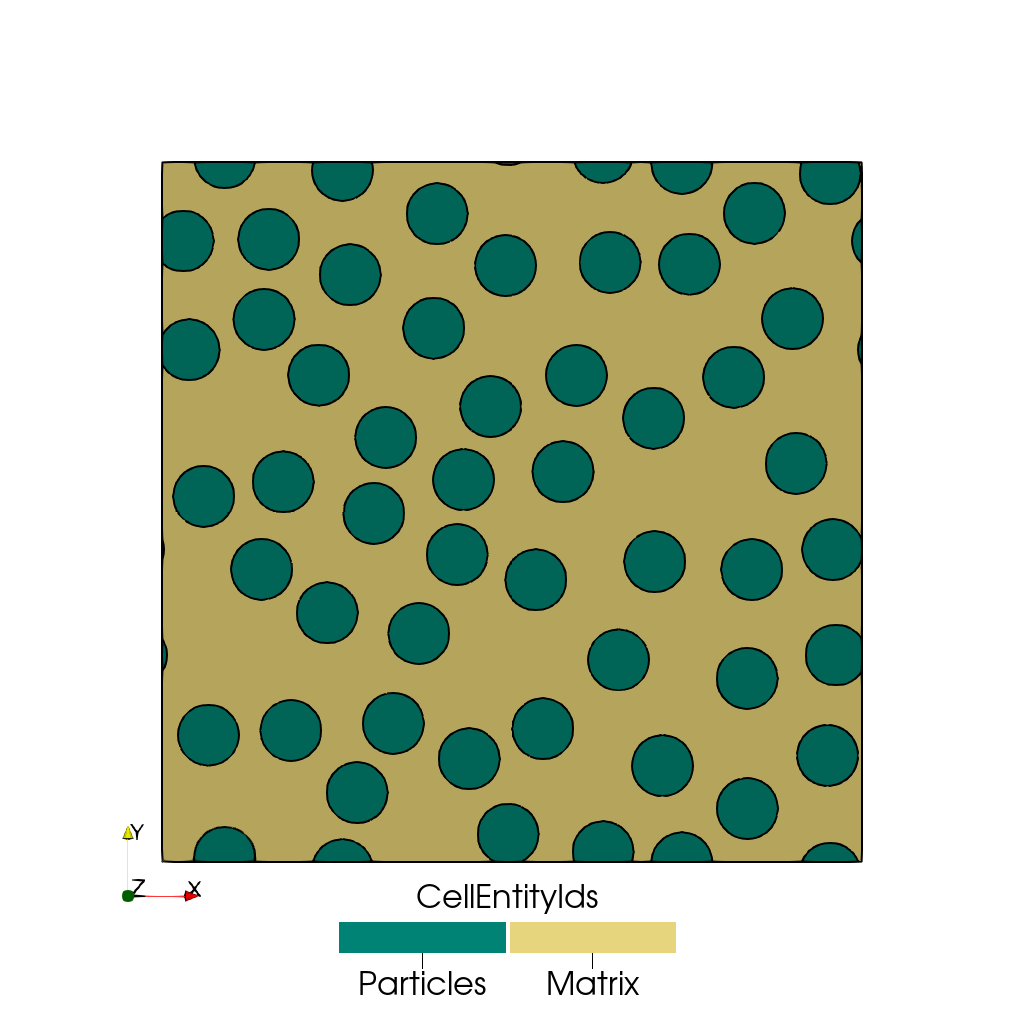
\includegraphics[width=\textwidth]{figures/2d_microstructure}
    \caption{}
    \label{subfig:2d_microstructure}
  \end{subfigure} \hfill
  \begin{subfigure}[b]{0.45\textwidth}
    \centering
    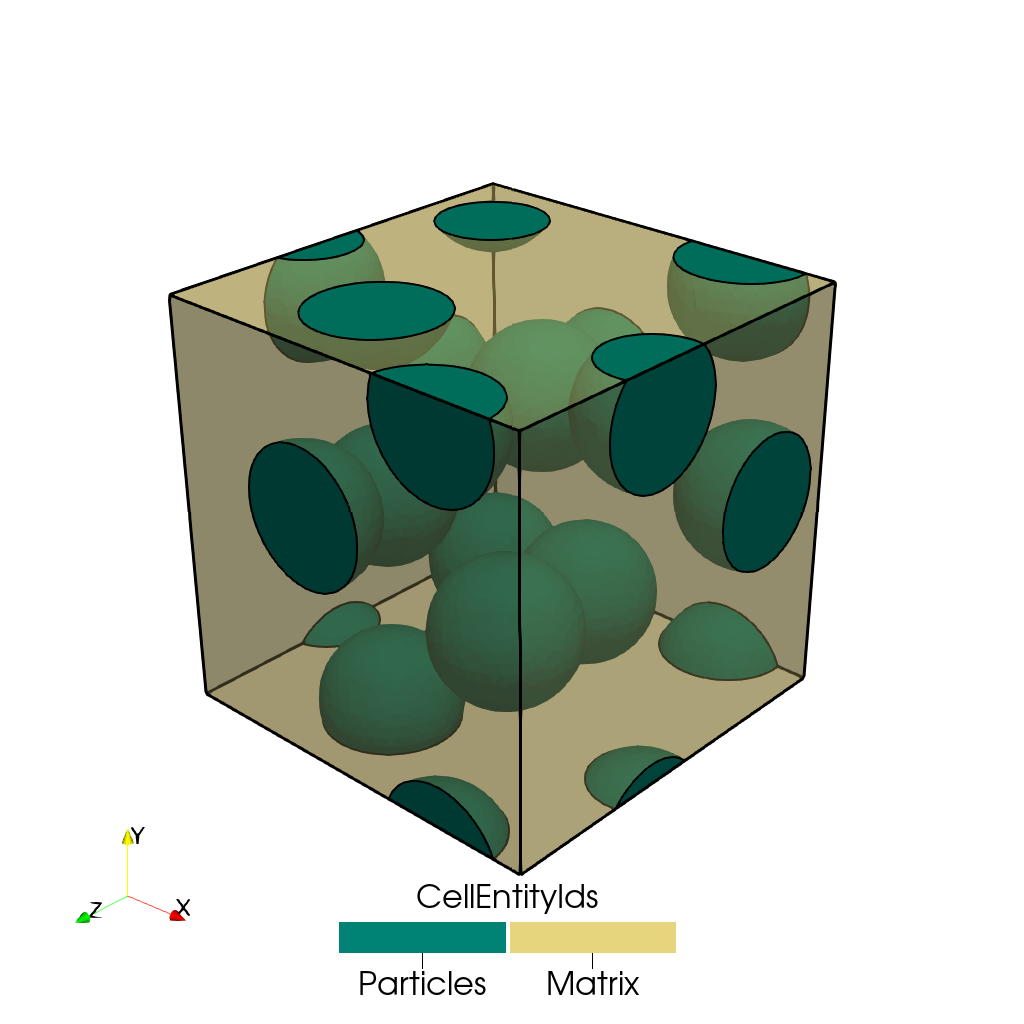
\includegraphics[width=\textwidth]{figures/3d_microstructure}
    \caption{}
    \label{subfig:3d_microstructure}
  \end{subfigure}
\caption{Dual phased heterogeneous materials microstructure: \subref{subfig:2d_microstructure} Fiber-reinforced composite (randomly distributed unidirectional circular cross-section fibers, \(f=30\%\)) - 2D RVE; \subref{subfig:3d_microstructure} Particle-reinforced composite (randomly distributed particles, \(f=20\%\)) - 3D RVE.}
\label{fig:microstructure}
\end{figure}



\subsection{Saint Venant-Kirchhoff model}

One of the simplest constitutive models to consider is a hyper-elastic model defined in the reference configuration.
Note that the problem is still non-linear because of the geometric nonlinearity.
According to \cite{de_geus_finite_2017} it can be described as follows.

\paragraph{Constitutive model}
The model is defined in the undeformed configuration and it involves a linear relation between the second Piola-Kirchhoff stress \(\boldsymbol{S}\) and the Green-Lagrange strain \(\boldsymbol{E}\)
\begin{equation} \label{eq:saint_venant_constitutive_equation}
\boldsymbol{S}=\boldsf{D}^e: \boldsymbol{E},
\end{equation}
wherein \(\boldsf{D}^e\) is the standard fourth-order elastic stiffness tensor
\begin{equation}
\boldsf{D}^e\equiv\lambda \boldsymbol{I} \otimes \boldsymbol{I}+2 \mu \boldsf{I}_{S},
\end{equation}
with Lamé's constants \(\lambda\) and \(\mu\). In terms of Young's modulus, \(E\), and Poisson's ratio, \(\nu\), they read
\begin{equation}
\lambda=\frac{E \nu}{(1+\nu)(1-2 \nu)}, \qquad \mu=\frac{E}{2(1+\nu)}.
\end{equation}
Furthermore, \(\boldsymbol{I}\) is the second-order identity tensor and \(\boldsf{I}_{S}\) is the fourth-order symmetrization tensor\footnote{The fourth order symmetrization tensor is defined as \({(\mathsf I_S)}_{ijkl} = \frac{1}{2}(\delta_{ik}\delta_{jl} + \delta_{il}\delta_{jk})\).}.

The connection to the deformation gradient tensor \(\boldsymbol{F}\) and the first Piola-Kirchhoff stress \(\boldsymbol{P}\) is made by the definition of the Green-Lagrange strain
\begin{equation}
\boldsymbol{E}=\frac{1}{2}\left(\boldsymbol{F}^{T}\boldsymbol{F}-\boldsymbol{I}\right),
\end{equation}
and of the first Piola-Kirchhoff stress
\begin{equation} \label{eq:stress_relation_saint_venant_kirchhoff}
\boldsymbol{P}=\boldsymbol{F} \boldsymbol{S}.
\end{equation}

\paragraph{Consistent tangent}
The constitutive model is linearized in the reference configuration in accordance with Equation~\eqref{eq:newton_increment}.
Its derivation is straightforward.
The first step is to linearize the stress relation in Equation~\eqref{eq:stress_relation_saint_venant_kirchhoff}, leading to
\begin{equation} \label{eq:saint_venant_kirchhoff_stress_lin}
\delta \boldsymbol{P}^{T}=\boldsymbol{S}^{(i)}\delta \boldsymbol{F}^{T}+\boldsf{I}_{R T}:\left(\boldsymbol{F}^{(i)}\delta \boldsymbol{S}\right),
\end{equation}
wherein \(\boldsf{I}_{R T}\) is the fourth-order right-transposed identity tensor\footnote{The fourth-order right-transposed identity tensor is defined as \((\mathsf I_{RT})_{ijkl} = \delta_{ik}\delta_{jl}\).}.
The constitutive model in Equation~\eqref{eq:saint_venant_constitutive_equation} is already linear.
Combined with the linearization of the Green-Lagrange strain one obtains
\begin{equation} \label{eq:saint_venant_kirchhoff_increment_2nd_piola}
\delta \boldsymbol{S}=\boldsf{D}^e:\left(\boldsf{I}^{s}{\boldsymbol{F}^{(i)}}^{T}\right): \delta \boldsymbol{F}.
\end{equation}
The expression of the tangent stiffness follows by combining Equations~\eqref{eq:saint_venant_kirchhoff_stress_lin} and \eqref{eq:saint_venant_kirchhoff_increment_2nd_piola} to obtain
\begin{equation}
\boldsf{A}^{(i)}=\boldsymbol{S}^{(i)}\boldsf{I}+\boldsf{I}_{R T}:\left(\boldsymbol{F}^{(i)}  \boldsf{D}^e  {\boldsymbol{F}^{(i)}}^{T}\right): \boldsf{I}_{R T},
\end{equation}
whereby the right-symmetry of \(\boldsf{D}^e\) has been used to absorb \(\boldsf{I}_{S}\).

\subsection{Hencky model}

The Hencky model is the finite logarithmic strain-based extension of the standard linear elastic material.
According to \cite{de2008computational} it can be described as follows.

\paragraph{Constitutive model}
Let \(\varepsilon\) be the Eulerian logarithmic strain tensor
\begin{equation} \label{eq:def_eulerian_log_strain}
\varepsilon \equiv \ln \boldsymbol{V}=\frac{1}{2} \ln \boldsymbol{B}.
\end{equation}
The Hencky strain-energy function is defined in compact form as
\begin{equation}
\bar{\rho} \psi(\varepsilon)=\frac{1}{2} \varepsilon: \boldsf{D}^e: \varepsilon,
\end{equation}
where \(\boldsf{D}^e\) has the format of the infinitesimal isotropic elasticity tensor
\begin{equation}
\boldsf{D}^e \equiv 2 G \boldsf{I}_{S}+\left(K-\frac{2}{3} G\right) \boldsymbol{I} \otimes \boldsymbol{I}.
\end{equation}

The above strain-energy renders the following linear relationship between the Kirchhoff stress and the Eulerian logarithmic strain
\begin{equation} \label{eq:hencky_stres_relation}
\bm\tau=\bar{\rho} \frac{\partial \psi}{\partial \varepsilon}=\boldsf{D}^e: \varepsilon,
\end{equation}
which has the same functional format as the infinitesimal linear elastic stress-strain relation.

\paragraph{Consistent tangent}

Under material isotropy, where \(\boldsymbol{\tau}\) can be expressed as a function of \(\boldsymbol{B}\) only, the spatial elasticity tensor can be equivalently represented as
\begin{equation} \label{eq:hecky_spatial_tangent_moduli_1st}
\boldsf{a}=\frac{2}{J} \frac{\partial \bm \tau}{\partial \bm B} \bm B-\boldsf{I}_{RT}\bm \sigma .
\end{equation}

As the Kirchhoff stress for the Hencky material is a linear function of the logarithmic Eulerian strain which, through its definition \eqref{eq:def_eulerian_log_strain}, is a function of \(B\), the derivative \(\partial \tau / \partial \boldsymbol{B}\) can be derived by a straightforward application of the chain rule to \eqref{eq:hencky_stres_relation}.
This gives
\begin{equation} \label{eq:hencky_1st_exp_for_deriv_tau_B}
\frac{\partial \boldsymbol{\tau}}{\partial \boldsymbol{B}}=\frac{\partial \boldsymbol{\tau}}{\partial \varepsilon}: \frac{\partial \varepsilon}{\partial \boldsymbol{B}}=\frac{1}{2} \boldsf{D}^e: \boldsf{L},
\end{equation}
where
\begin{equation}
\boldsf{L} \equiv \frac{\partial(\ln \boldsymbol{B})}{\partial \boldsymbol{B}},
\end{equation}
is the derivative of the tensor logarithm function evaluated at \(\bm B\).

In order to derive a compact expression for the Hencky elasticity tensor, we note that \eqref{eq:hecky_spatial_tangent_moduli_1st} is equivalent to
\begin{equation} \label{eq:hecky_spatial_tangent_moduli_2nd}
\boldsf{a}=\frac{1}{J}\frac{\partial \boldsymbol{\tau}}{\partial \boldsymbol{B}}: \boldsf{B}-\boldsf{I}_{RT}\bm\sigma
\end{equation}
where we have defined the fourth-order tensor \(\boldsf{B}\) by
\begin{equation}
\boldsf{B} \equiv 2\boldsf{I}_S \bm B.
\end{equation}
Finally, formula \eqref{eq:hecky_spatial_tangent_moduli_2nd} together with \eqref{eq:hencky_1st_exp_for_deriv_tau_B} yields the following expression for the Hencky spatial elasticity tensor
\begin{equation}
\boldsf{a}=\frac{1}{2 J}\boldsf{D}^e: \boldsf{L}: \boldsf{B}-\boldsf{I}_{RT}\bm\sigma,
\end{equation}
which has a particularly simple format.
The pull-back\textcolor{red}{(?)} to the material configuration is given by
\begin{equation}
  \boldsf{A}^{(i)} = {\bm F^{(i)}}^{-1}\left(\frac{1}{2}\boldsf{D}^e:{\boldsf L}^{(i)}: {\boldsf B}^{(i)} - \boldsf{I}_{RT}\bm \tau^{(i)}\right){\bm F^{(i)}}^{-T},
\end{equation}
reintroducing the dependency on the current Newton iteration \((i)\).

\section{Comparison between FFT and FEM-based homogenization}


To better gauge the accuracy and efficiency of the FFT-based Galerkin formulation, some numerical simulations are performed.
Their goals is to (1) validate the implementation of the FFT-based homogenization Galerkin scheme \citep{vondrejc_fft-based_2014, zeman_finite_2017, de_geus_finite_2017}, (2) compare the accuracy and computational performance between the FFT, basic \citep{moulinec_fast_1994} and Galerkin formulation, and FEM-based homogenization approaches and (3) choose the suitable spatial discretization refinement to evaluate the microstructures in Figure~\ref{fig:microstructure}.

Concerning the FFT-based homogenization, the same discretization is performed in the different problem dimensions \(\left(n_{v, 1}=n_{v, 2}=n_{v, 3}\right)\).
In order to generate the FEM finite element meshes, the FFT-FEM mesh conversion strategy adopted is to convert the pixels (2D) and voxels (3D) into quadrilateral (2D) and brick (3D) finite elements.
It is employed with both linear (QUAD4, HEXA8) and quadratic finite elements (QUAD8, HEXA20) such that \(n_{e}=n_{v}\).
Moreover, given the solver library available in LINKS, two types of solvers are considered in the FEM-based homogenization simulations: the direct solver MKL PARDISO \citep{schenk2001pardiso, schenk2004solving} and the iterative solver WSMP (Watson Sparse Matrix Package) \citep{gupta_improved_2002, gupta_wsmp_2002} with an SSOR (Symmetric Successive Over-relaxation) preconditioner.
Extensive preliminary research has shown that these are the overall (solver time and memory footprint) best direct and iterative solvers available in Links \citep{cardoso_coelho_election_2019}.

\subsection{Small strain}

\paragraph{Comparison of the convergence criteria}
The following numerical results are obtained to provide a better understanding of the differences in efficiency and accuracy between the two convergence criteria detailed in Section~\ref{sec:criteria}.

Both phases are assumed linear elastic (see Table~\ref{tab:mat_properties} for the properties), periodic boundary conditions are adopted and the following macroscale strain loading case is considered
\begin{equation}
\text { uniaxial: } \bm{\varepsilon}=\left[\begin{array}{lll}
5 & 0 & 0 \\
0 & 0 & 0 \\
0 & 0 & 0
\end{array}\right] \times 10^{-3}
\end{equation}
being enforced in a single load increment.
Note that in the 2D plane strain case, only the inplane \(O_{x y}\) macroscale strain components are enforced.

The numerical results of the fiber-reinforced linear elastic composite equilibrium problem using the two criteria under analysis are shown in Figure~\ref{fig:linear_2D_normal_comparison_crit} for the uniaxial loading case.
Figure~\ref{subfig:linear_2D_normal_comparison_crit_homo_stress_11_vs_n_voxels} shows that both FFT techniques converge to the same value at approximately the same rate as a function of the number of voxels in the discritization.
Also, no noticeable difference can be seen between the two convergence criteria considered.
Regarding the CPU time expended to reach an error of \num{1e-6}, presented in Figure~\ref{subfig:linear_2D_normal_comparison_crit_cpu_time_vs_n_voxels}, Criterion I leads to faster convergence.
This effect is stronger for the FFT Basic scheme.

\begin{figure}[hbt] % fig:linear_2D_normal_comparison_crit
  \centering
	\begin{subfigure}[b]{0.51\textwidth}
    \centering
    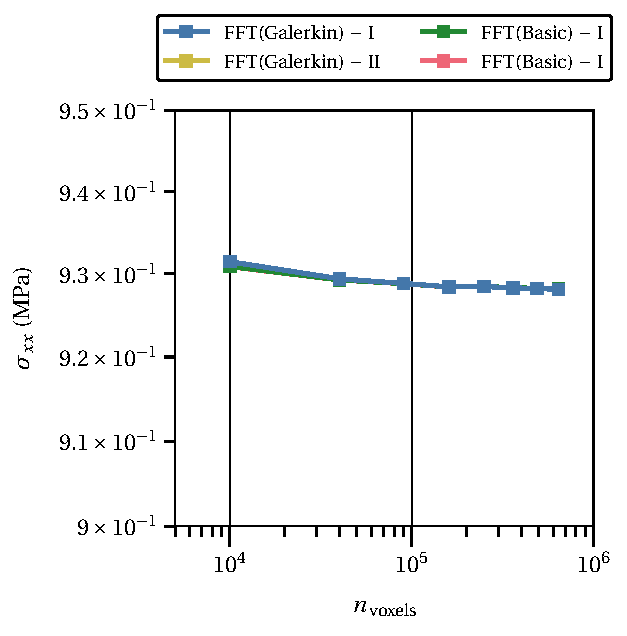
\includegraphics[width=\textwidth]{figures/linear_2D_normal_comparison_crit_homo_stress_11_vs_n_voxels}
    \caption{}
    \label{subfig:linear_2D_normal_comparison_crit_homo_stress_11_vs_n_voxels}
  \end{subfigure}
  \begin{subfigure}[b]{0.48\textwidth}
    \centering
    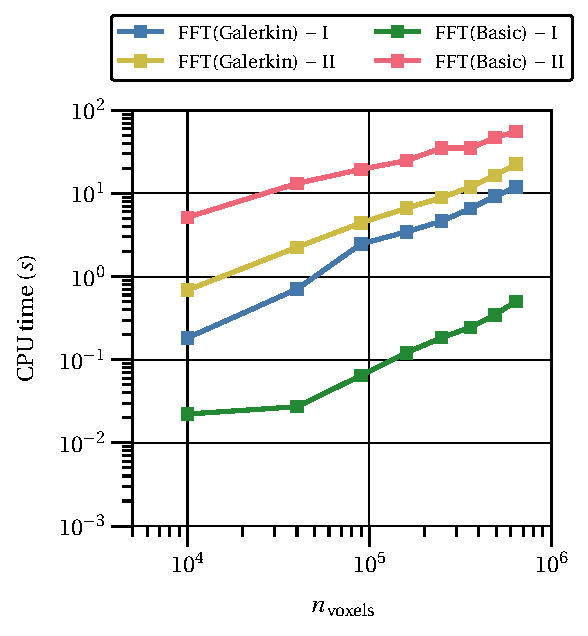
\includegraphics[width=\textwidth]{figures/linear_2D_normal_comparison_crit_cpu_time_vs_n_voxels}
    \caption{}
    \label{subfig:linear_2D_normal_comparison_crit_cpu_time_vs_n_voxels}
  \end{subfigure}
  \caption{Comparison between the Criterion I and II for FFT-based homogenization
  approaches, Galerkin and Basic, in the solution of the fiber-reinforced linear elastic
  composite equilibrium problem under uniaxial strain loading conditions:
  \subref{subfig:linear_2D_normal_comparison_crit_homo_stress_11_vs_n_voxels} Homogenized
  stress; \subref{subfig:linear_2D_normal_comparison_crit_cpu_time_vs_n_voxels}
  Computational time.}
  \label{fig:linear_2D_normal_comparison_crit}
\end{figure}

The numerical results of the particle-reinforced linear elastic composite equilibrium problem are shown in Figure~\ref{fig:linear_3D_normal_comparison_crit} for the uniaxial loading case.
The results mirror the ones found for the two-dimensional example.
Figure~\ref{subfig:linear_3D_normal_comparison_crit_homo_stress_11_vs_n_voxels} shows that both FFT techniques converge to the same value at approximately the same rate as a function of the number of voxels in the discritization.
Also, no noticeable difference can be seen between the two convergence criteria considered.
Regarding the CPU time expended to reach an error of \num{1e-5}, presented in Figure~\ref{subfig:linear_3D_normal_comparison_crit_cpu_time_vs_n_voxels}, Criterion I leads to faster convergence.
This effect is stronger for the FFT Basic scheme.

\begin{figure}[hbt] % fig:linear_3D_normal_comparison_crit
  \centering
	\begin{subfigure}[b]{0.52\textwidth}
    \centering
    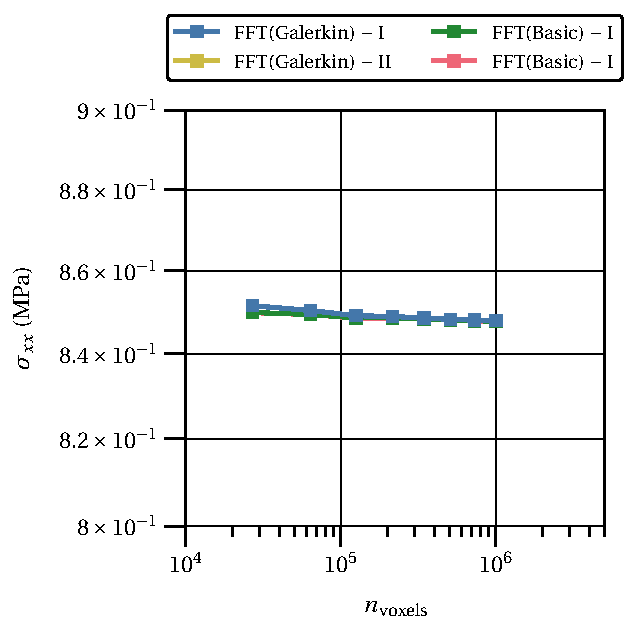
\includegraphics[width=\textwidth]{figures/linear_3D_normal_comparison_crit_homo_stress_11_vs_n_voxels}
    \caption{}
    \label{subfig:linear_3D_normal_comparison_crit_homo_stress_11_vs_n_voxels}
  \end{subfigure}
  \begin{subfigure}[b]{0.46\textwidth}
    \centering
    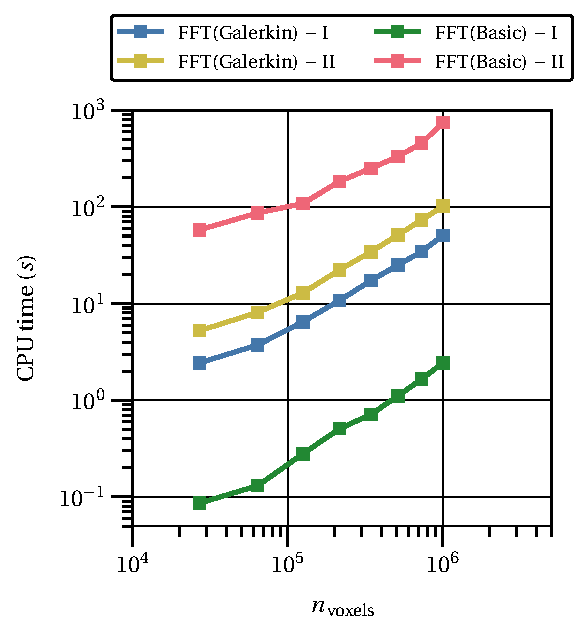
\includegraphics[width=\textwidth]{figures/linear_3D_normal_comparison_crit_cpu_time_vs_n_voxels}
    \caption{}
    \label{subfig:linear_3D_normal_comparison_crit_cpu_time_vs_n_voxels}
  \end{subfigure}
  \caption{Comparison between the Criterion I and II for FFT-based homogenization
  approaches, Galerkin and Basic, in the solution of the particle-reinforced linear elastic
  composite equilibrium problem under uniaxial strain loading conditions:
  \subref{subfig:linear_3D_normal_comparison_crit_homo_stress_11_vs_n_voxels} Homogenized
  stress; \subref{subfig:linear_3D_normal_comparison_crit_cpu_time_vs_n_voxels}
  Computational time.} \label{fig:linear_3D_normal_comparison_crit}
\end{figure}

\FloatBarrier

\paragraph{Accuracy validation}
Both phases are assumed linear elastic (see Table~\ref{tab:mat_properties} for the properties), periodic boundary conditions are adopted and the following two macroscale strain loading cases are considered
\begin{equation}
\text { uniaxial: } \bm{\varepsilon}=\left[\begin{array}{lll}
5 & 0 & 0 \\
0 & 0 & 0 \\
0 & 0 & 0
\end{array}\right] \times 10^{-3}, \quad \text { pure shear: } \quad \bm \varepsilon=\left[\begin{array}{ccc}
0 & 5 & 5 \\
5 & 0 & 5 \\
5 & 5 & 0
\end{array}\right] \times 10^{-3},
\end{equation}
being enforced in a single load increment.
Note that in the 2D plane strain case, only the inplane \(O_{x y}\) macroscale strain components are enforced.
The convergence criterion used is Criterion II, as described in Section~\ref{sec:criteria}.

The numerical results of the fiber-reinforced linear elastic composite equilibrium problem are shown in Figures~\ref{fig:linear_2D_normal} and \ref{fig:shear_2D_normal} for the uniaxial and pure shear loading cases, respectively.
In both cases there is an excellent agreement between the FFT and FEM-based homogenization solutions concerning both the homogenized response (see Figures~\ref{subfig:linear_2D_normal_homo_stress_11_vs_n_voxels} and \ref{subfig:linear_2D_shear_homo_stress_12_vs_n_voxels} and the local strain fields (see Figures \ref{subfig:linear_2D_normal_strain_11} and \ref{subfig:linear_2D_shear_strain_12}.
In terms of computational performance, Figures~\ref{subfig:linear_2D_normal_cpu_time_vs_n_voxels} and \ref{subfig:linear_2D_shear_cpu_time_vs_n_voxels} show that the FFT-based homogenization Galerkin scheme outperforms the FEM-based homogenization with speedups of around 2 relative to the direct solver with linear finite elements.
There is however a caveat, regarding this direct comparison.
The Python libraries used in the implementation of the FFT-based homogenization Galerkin scheme are parallelized and used all the cores available in the machine at the time.
On the other hand, the FEM simulations are run using only one core.
When compared with the FFT-based homogenization basic scheme, the CPU time expended differs by more than an order of magnitude, with the Galerkin scheme being slower.

\begin{figure}[hbt] % fig:linear_2D_normal
  \centering
	\begin{subfigure}[b]{0.49\textwidth}
    \centering
    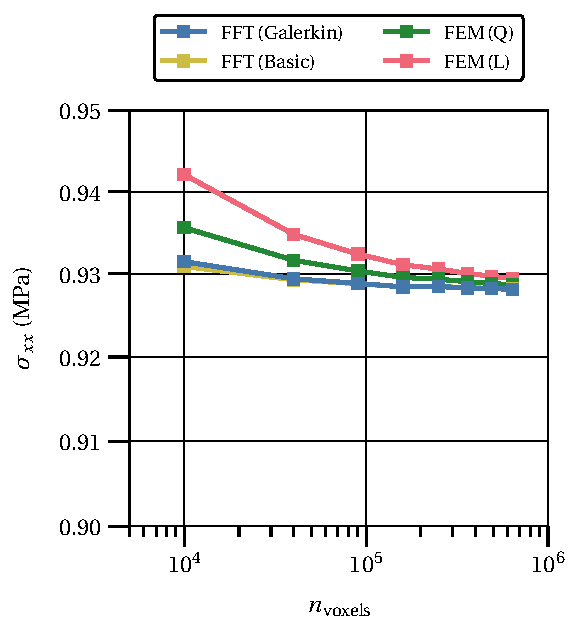
\includegraphics[width=\textwidth]{figures/linear_2D_normal_homo_stress_11_vs_n_voxels}
    \caption{}
    \label{subfig:linear_2D_normal_homo_stress_11_vs_n_voxels}
  \end{subfigure}
  \begin{subfigure}[b]{0.49\textwidth}
    \centering
    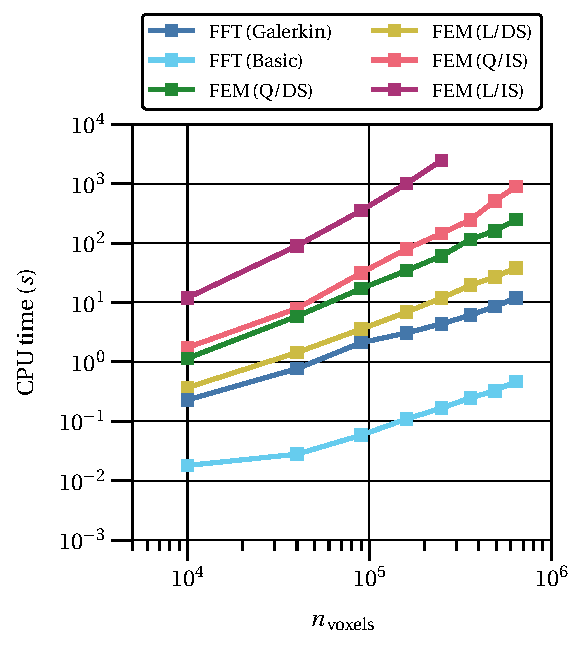
\includegraphics[width=\textwidth]{figures/linear_2D_normal_cpu_time_vs_n_voxels}
    \caption{}
    \label{subfig:linear_2D_normal_cpu_time_vs_n_voxels}
  \end{subfigure}
  \begin{subfigure}[b]{\textwidth}
    \centering
    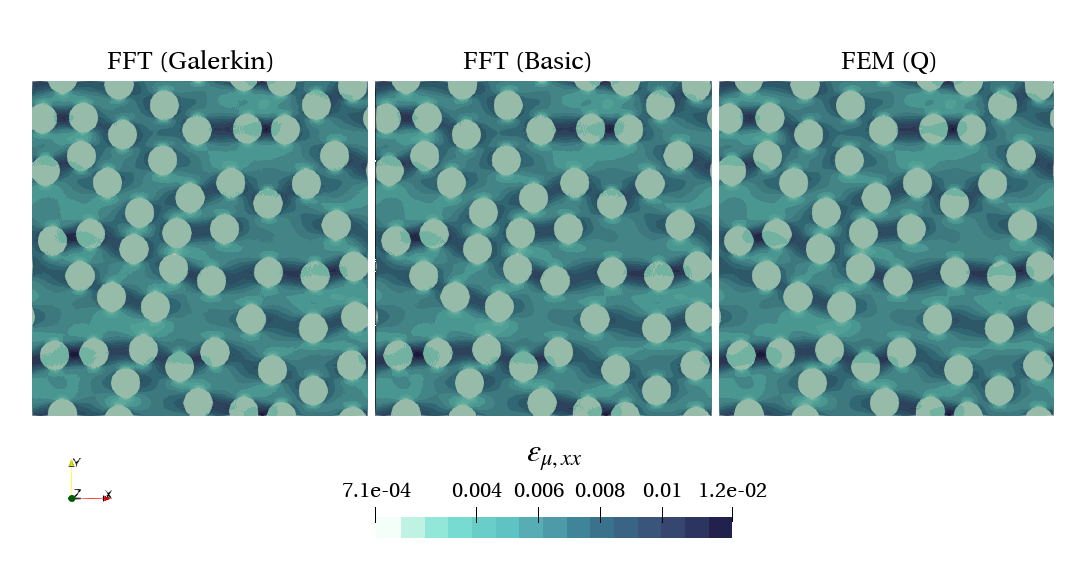
\includegraphics[width=\textwidth]{figures/linear_2D_normal_strain_11}
    \caption{}
    \label{subfig:linear_2D_normal_strain_11}
  \end{subfigure}
  \caption{Comparison between the FFT and FEM-based homogenization approaches in the
  solution of the fiber-reinforced linear elastic composite equilibrium problem under pure
  shear strain loading conditions:
  \subref{subfig:linear_2D_normal_homo_stress_11_vs_n_voxels} Homogenized stress;
  \subref{subfig:linear_2D_normal_cpu_time_vs_n_voxels} Computational time;
  \subref{subfig:linear_2D_normal_strain_11} Local strain field (\(n_v = 600 \times 600\)
  discretization). Notation: linear element (L), quadratic element (Q), direct solver (DS)
  and iterative solver (IS)}
  \label{fig:linear_2D_normal}
\end{figure}

\begin{figure}[hbt] % fig:linear_2D_shear
  \centering
	\begin{subfigure}[b]{0.49\textwidth}
    \centering
    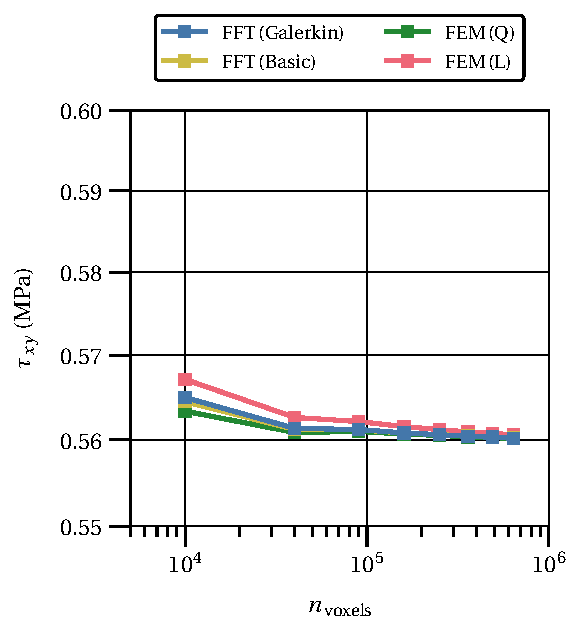
\includegraphics[width=\textwidth]{figures/linear_2D_shear_homo_stress_12_vs_n_voxels}
    \caption{}
    \label{subfig:linear_2D_shear_homo_stress_12_vs_n_voxels}
  \end{subfigure}
  \begin{subfigure}[b]{0.49\textwidth}
    \centering
    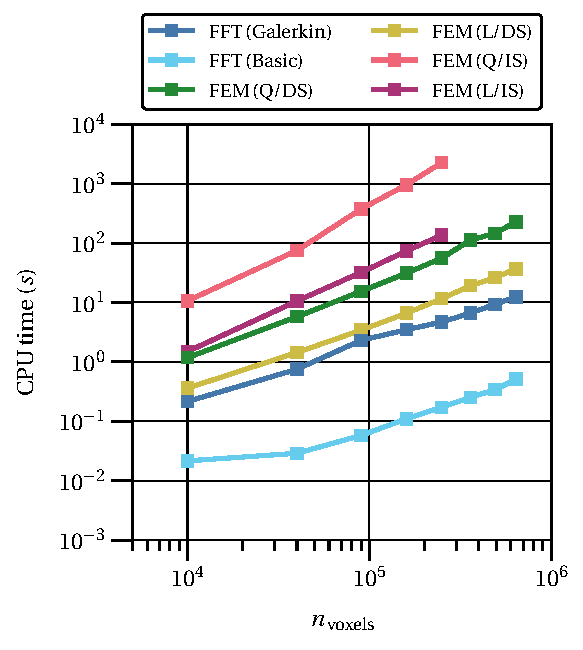
\includegraphics[width=\textwidth]{figures/linear_2D_shear_cpu_time_vs_n_voxels}
    \caption{}
    \label{subfig:linear_2D_shear_cpu_time_vs_n_voxels}
  \end{subfigure}
  \begin{subfigure}[b]{\textwidth}
    \centering
    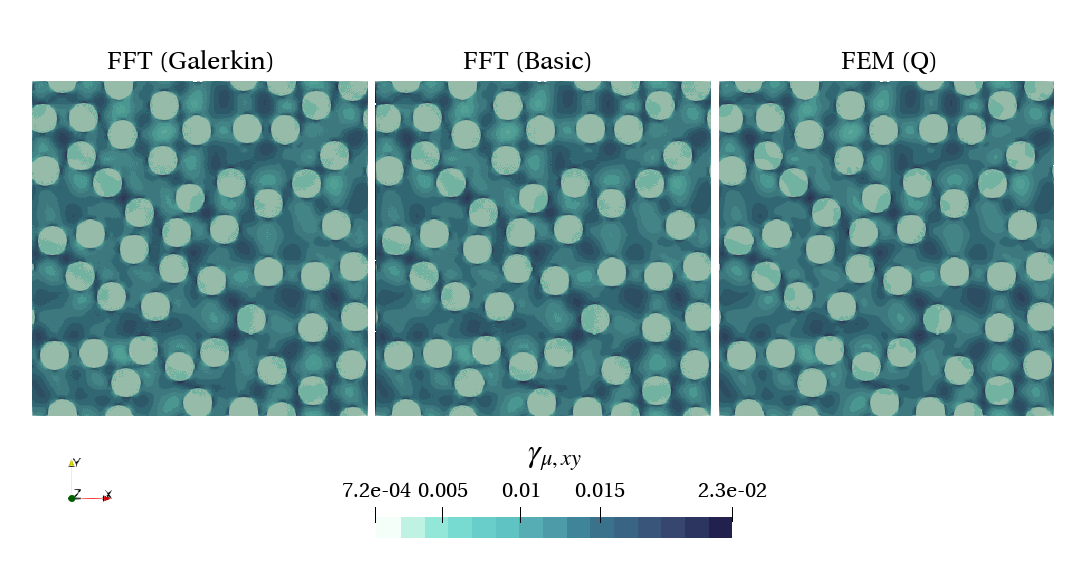
\includegraphics[width=\textwidth]{figures/linear_2D_shear_strain_12}
    \caption{}
    \label{subfig:linear_2D_shear_strain_12}
  \end{subfigure}
  \caption{Comparison between the FFT and FEM-based homogenization approaches in the
  solution of the fiber-reinforced linear elastic composite equilibrium problem under pure
  shear strain loading conditions:
  \subref{subfig:linear_2D_normal_homo_stress_11_vs_n_voxels} Homogenized stress;
  \subref{subfig:linear_2D_normal_cpu_time_vs_n_voxels} Computational time;
  \subref{subfig:linear_2D_normal_strain_11} Local strain field (\(n_v = 600 \times 600\)
  discretization). Notation: linear element (L), quadratic element (Q), direct solver (DS)
  and iterative solver (IS)}
  \label{fig:linear_2D_shear}
\end{figure}

The numerical results of the particle-reinforced linear elastic composite equilibrium problem are shown in Figures~\ref{fig:linear_3D_normal} and \ref{fig:linear_3D_shear} for the uniaxial and pure shear loading cases, respectively.
Once again there is an excellent agreement between the FFT and FEM-based homogenization solutions concerning both the homogenized response (see Figures \ref{subfig:linear_3D_normal_homo_stress_11_vs_n_voxels} and \ref{subfig:linear_3D_shear_homo_stress_12_vs_n_voxels} and the local strain fields (see Figures~\ref{subfig:linear_3D_normal_strain_11} and \ref{subfig:linear_3D_shear_strain_12}.
In terms of computational performance, Figures~\ref{subfig:linear_3D_normal_cpu_time_vs_n_voxels} and \ref{subfig:linear_3D_shear_cpu_time_vs_n_voxels} show that the FFT-based homogenization Galerkin scheme outperforms the FEM-based homogenization with speedups ranging from around 10 and 100 relative to the iterative solver with linear and quadratic finite elements, respectively.
The same remark concerning the number of cores used in each method mention previous also applies here.
Comparing the two FFT-based schemes, the basic scheme is faster by an order of magnitude than Galerkin scheme.
Adding to this, the 3D cases highlight another important aspect concerning FEM-based homogenization. When attempting to run the direct solver simulations with \(n_{e}=80 \times 80 \times 80\) (linear finite element mesh) and \(n_{e}=50 \times 50 \times 50\) (quadratic finite element mesh) the memory required to build the global tangent stiffness matrix (stored in compressed sparse row (CSR) format) exceeds the available 128 GB!
Despite reaching a significantly lower peak memory than the direct solver, the iterative solver suffered from the same limitation for a simulation over \(n_{e}=100 \times 100 \times 100\) (linear finite element mesh) and \(n_{e}=70 \times 70 \times 70\) (quadratic finite element mesh).
In comparison, the FFT-based homogenization memory footprint is almost negligible as it does not require the computation of a global tangent stiffness matrix.

\begin{figure}[hbt] % fig:linear_3D_normal
  \centering
	\begin{subfigure}[b]{0.49\textwidth}
    \centering
    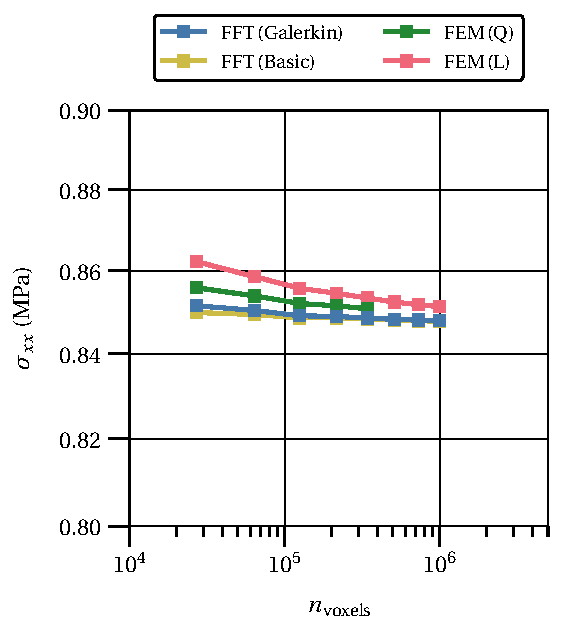
\includegraphics[width=\textwidth]{figures/linear_3D_normal_homo_stress_11_vs_n_voxels}
    \caption{}
    \label{subfig:linear_3D_normal_homo_stress_11_vs_n_voxels}
  \end{subfigure}
  \begin{subfigure}[b]{0.49\textwidth}
    \centering
    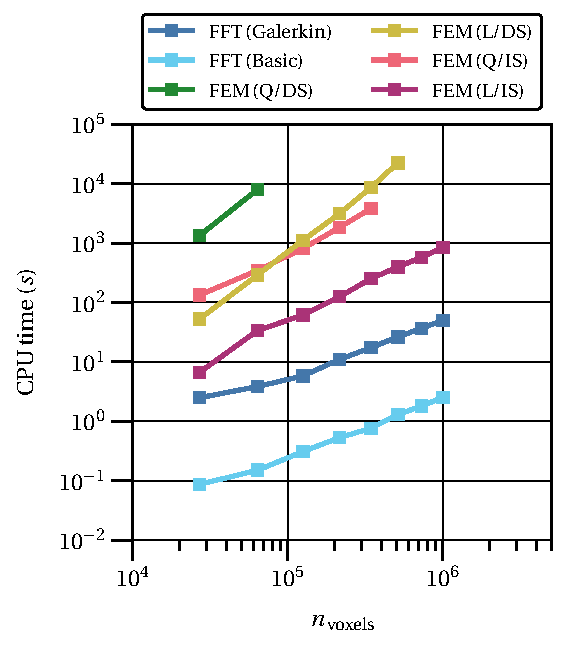
\includegraphics[width=\textwidth]{figures/linear_3D_normal_cpu_time_vs_n_voxels}
    \caption{}
    \label{subfig:linear_3D_normal_cpu_time_vs_n_voxels}
  \end{subfigure}
  \begin{subfigure}[b]{\textwidth}
    \centering
    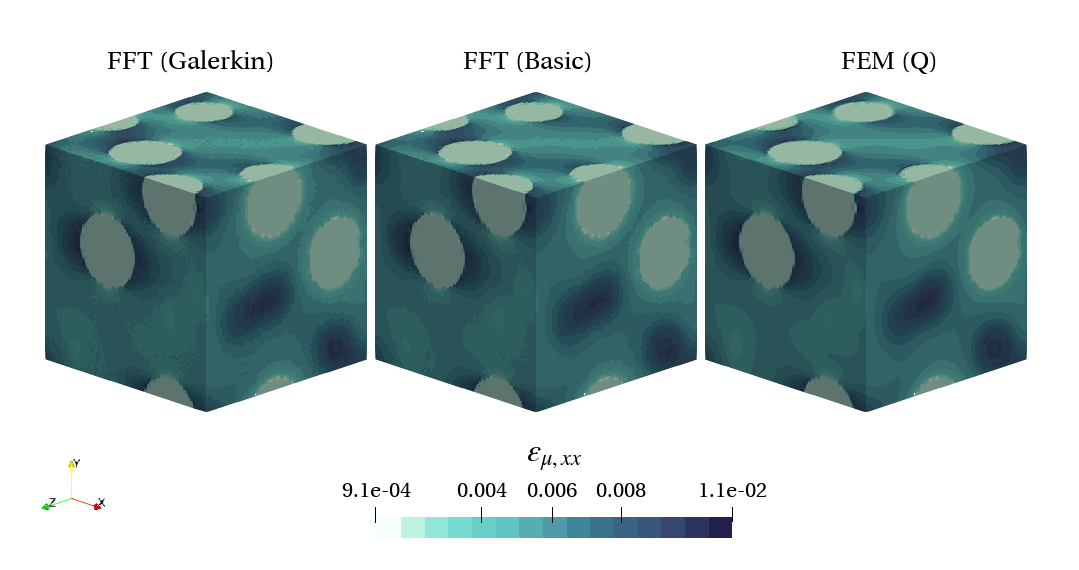
\includegraphics[width=\textwidth]{figures/linear_3D_normal_strain_11}
    \caption{}
    \label{subfig:linear_3D_normal_strain_11}
  \end{subfigure}
  \caption{Comparison between the FFT and FEM-based homogenization approaches in the
  solution of the particle-reinforced linear elastic composite equilibrium problem under normal
  strain loading conditions: \subref{subfig:linear_3D_normal_homo_stress_11_vs_n_voxels} Homogenized stress; \subref{subfig:linear_3D_normal_cpu_time_vs_n_voxels} Computational time; \subref{subfig:linear_3D_normal_strain_11} Local strain field
  (\(n_v = 70 \times 70\times 70\) discretization). Notation: linear element (L), quadratic element (Q), direct solver
  (DS) and iterative solver (IS)}
  \label{fig:linear_3D_normal}
\end{figure}

\begin{figure}[hbt] % fig:linear_3D_shear
  \centering
	\begin{subfigure}[b]{0.49\textwidth}
    \centering
    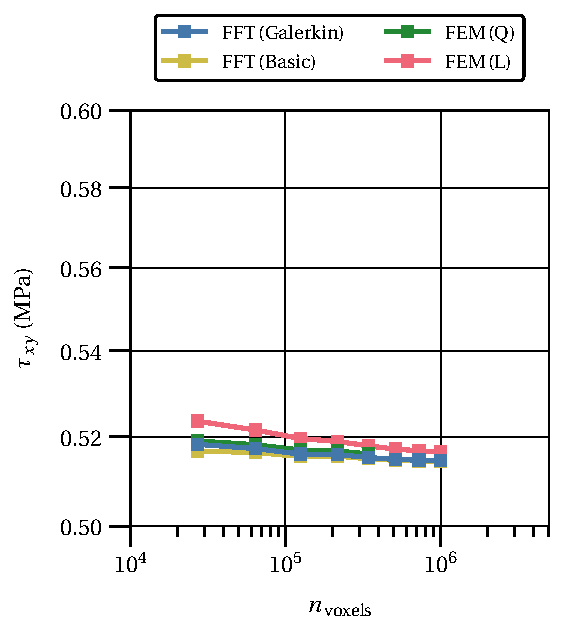
\includegraphics[width=\textwidth]{figures/linear_3D_shear_homo_stress_12_vs_n_voxels}
    \caption{}
    \label{subfig:linear_3D_shear_homo_stress_12_vs_n_voxels}
  \end{subfigure}
  \begin{subfigure}[b]{0.49\textwidth}
    \centering
    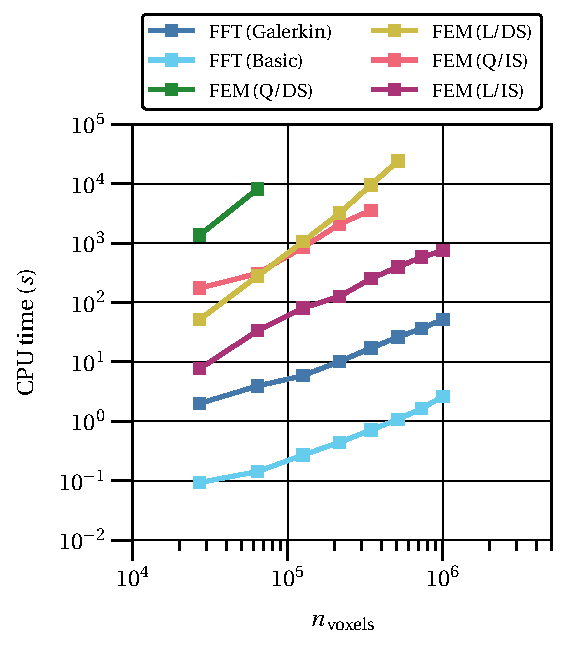
\includegraphics[width=\textwidth]{figures/linear_3D_shear_cpu_time_vs_n_voxels}
    \caption{}
    \label{subfig:linear_3D_shear_cpu_time_vs_n_voxels}
  \end{subfigure}
  \begin{subfigure}[b]{\textwidth}
    \centering
    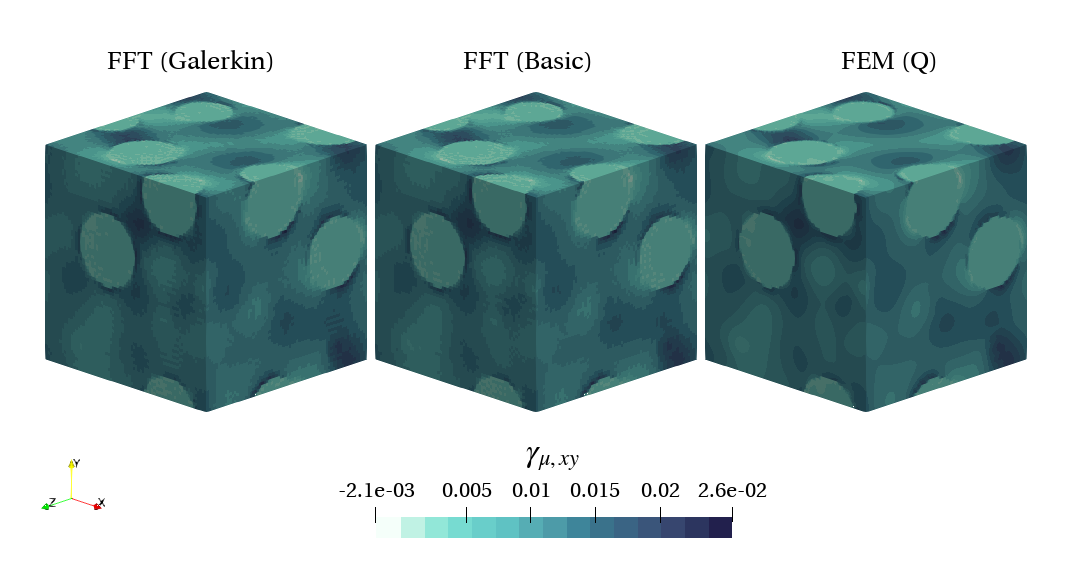
\includegraphics[width=\textwidth]{figures/linear_3D_shear_strain_12}
    \caption{}
    \label{subfig:linear_3D_shear_strain_12}
  \end{subfigure}
  \caption{Comparison between the FFT and FEM-based homogenization approaches in the
  solution of the fiber-reinforced linear elastic composite equilibrium problem under pure shear
  strain loading conditions: \subref{subfig:linear_3D_shear_homo_stress_12_vs_n_voxels} Homogenized stress; \subref{subfig:linear_3D_normal_cpu_time_vs_n_voxels} Computational time; \subref{subfig:linear_3D_normal_strain_11} Local strain field
  (\(n_v = 70 \times 70 \times 70\) discretization). Notation: linear element (L), quadratic element (Q), direct solver
  (DS) and iterative solver (IS).}
  \label{fig:linear_3D_shear}
\end{figure}

From the results present, a few conclusions and remarks are in order:
\begin{itemize}
  \item The FFT-based homogenization Galerkin scheme implementation is validated as solutions obtained (both homogenized results and local fields) are in excellent agreement with ones obtained with the FEM-based homogenization from LINKS and the FFT-based homogenization basic scheme;
  \item In the linear elastic regime, the FFT-based homogenization Galerkin scheme outperforms the FEM-based homogenization both in terms of speed and memory footprint.
  However, it must be kept in the mind that some of the Python libraries employed in the implementation of the FFT-based homogenization Galerkin scheme are parallelized and only one core was used in the LINKS simulations.
  \item In the linear elastic regime, the FFT-based homogenization basic scheme outperforms the FFT-based homogenization Galerkin scheme in terms of CPU time expended.
  Yet, consider that the implementation of the basic scheme used in the comparison \cite{} has already undergone some perfomance optimization.
  This is not the case for the Galerkin scheme.
  \item Given the solution convergence with the increasing sampling/meshing refinement, the spatial discretizations of \(n_{v}=600 \times 600\) (fiber-reinforced composite 2D RVE) and \(n_{v}=70 \times\) \(70 \times 70\) (particle-reinforced composite 3D RVE) are considered hereafter unless otherwise stated;
  \item In the following numerical studies, the reference DNS solution is obtained considering quadratic finite elements (QUAD8 and HEXA20) and the fastest solver time (MKL PARDISO in the 2D case and WSMP-SSOR in the \(3 \mathrm{D}\) case) unless otherwise stated.
\end{itemize}

\FloatBarrier

\paragraph{Extreme stiffness ratios between phases}

The following set of results is presented to better comprehend the limitations of the FFT-based methods regarding the stiffness ratio between the phases, widely reported in the literature \cite{}.
As previously, FEM solutions are used as a standard.

Both phases are assumed linear elastic having the same Poisson's ratio, \(\nu=0.3\).
The Young modulus of the matrix is fixed at \(E_1=\SI{100}{\mega\pascal}\) and the ratio between the stiffness of the particles and the matrix, \(K=E_1/E_2\), is made to vary from \num{e-6} to \num{e4} in increments of \(\times \sqrt{10}\).
Periodic boundary conditions are adopted and the following macroscale strain loading case is considered
\begin{equation}
\text { uniaxial: } \bm{\varepsilon}=\left[\begin{array}{lll}
5 & 0 & 0 \\
0 & 0 & 0 \\
0 & 0 & 0
\end{array}\right] \times 10^{-3},
\end{equation}
being enforced in a single load increment.
Note that in the 2D plane strain case, only the inplane \(O_{x y}\) macroscale strain components are enforced.

The numerical results of the fiber-reinforced linear elastic composite equilibrium problem are shown in Figures~\ref{fig:linear_2D_normal_stiff_contrast} for the uniaxial loading case.
There is an excellent agreement between the FFT and FEM-based homogenization solutions concerning the homogenized response as attested by Figure~\ref{subfig:linear_2D_normal_stress_avg_vs_stiff_ratio}.
In terms of computational performance, Figure~\ref{subfig:linear_2D_normal_stress_avg_cpu_time_vs_n_voxels} shows that the FFT-based homogenization Galerkin scheme outperforms the FEM-based homogenization with speedups from around 20 at low stiffness contrast to around 2 at the hightest stiffness contrasts, both high and low, relative to the direct solver with linear finite elements.
As before, the caveat regarding the parallelization of the Python libraries still applies.
When compared with the FFT-based homogenization basic scheme, the CPU time expended differs from one to two orders of magnitude across the stiffness ranges considered, with the Galerkin scheme being slower.
However, the basic scheme is unable to reach the preset tolerance \((\num{e-6})\) for stiffness ratios beyond the range \([\num{e-3},\num{e3}]\).

Concerning the local field, an excellent agreement can be observed at both high \((K=E_1/E_2=\num{e4})\) and low \((K=E_1/E_2=\num{e-4})\) stiffness ratios in the matrix phase, as can be seen in Figures~\ref{fig:linear_2D_stiff_contrast_normal_strain_11} and \ref{fig:linear_2D_stiff_contrast_normal_stress_11}.
There is also good agreement regarding the local field in the particle phase for the strain field at the low stiffness ratio and the stress field at the high stiffness ratio.
On the other hand, the strain field at the low stiffness ratio and the strain field at the high stiffness ratio exihibt strong oscillations in the particle phase.
This phenomenon is often denominated by "ringing" and is widely reported in the literature as being a consequence of very high or low stiffness ratios.
Figure~\ref{} provides a more detailed representation of the variation of the strain field \(\varepsilon_{\mu,xx}\) inside the particle pahse at a stiffness ratio equal to \num{e-4}.


\begin{figure}[hbt]
  \centering
  	\begin{subfigure}[b]{0.49\textwidth}
      \centering
      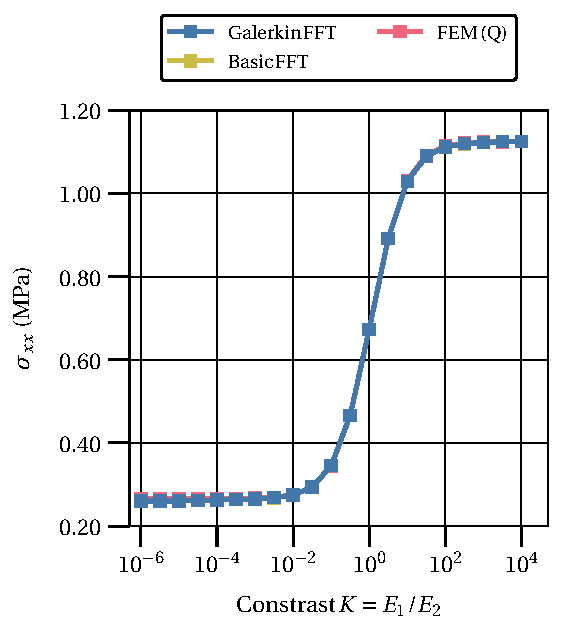
\includegraphics[width=\textwidth]{figures/linear_2D_normal_stress_avg_vs_stiff_ratio}
      \caption{}
      \label{subfig:linear_2D_normal_stress_avg_vs_stiff_ratio}
    \end{subfigure}
    \begin{subfigure}[b]{0.49\textwidth}
      \centering
      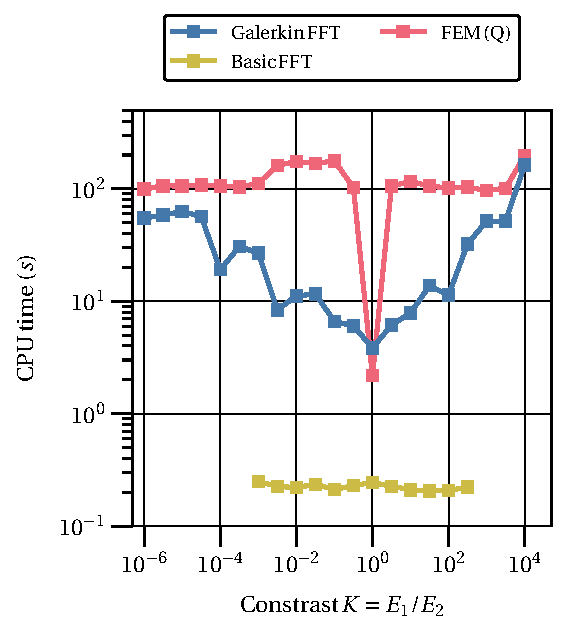
\includegraphics[width=\textwidth]{figures/linear_2D_normal_stress_avg_cpu_time_vs_n_voxels}
      \caption{}
      \label{subfig:linear_2D_normal_stress_avg_cpu_time_vs_n_voxels}
    \end{subfigure}
  \caption{Comparison between the FFT and FEM-based homogenization approaches in the solution
  of the fiber-reinforced linear elastic composite equilibrium problem under normal strain
  loading conditions: \subref{subfig:linear_2D_normal_stress_avg_vs_stiff_ratio} Homogenized
  stress; \subref{subfig:linear_2D_normal_stress_avg_cpu_time_vs_n_voxels} Computational time;
  Notation: linear element (L), quadratic element (Q).}
\label{fig:linear_2D_normal_stiff_contrast}
\end{figure}

\begin{figure}[hbt]
  \centering
	\begin{subfigure}[b]{\textwidth}
    \centering
    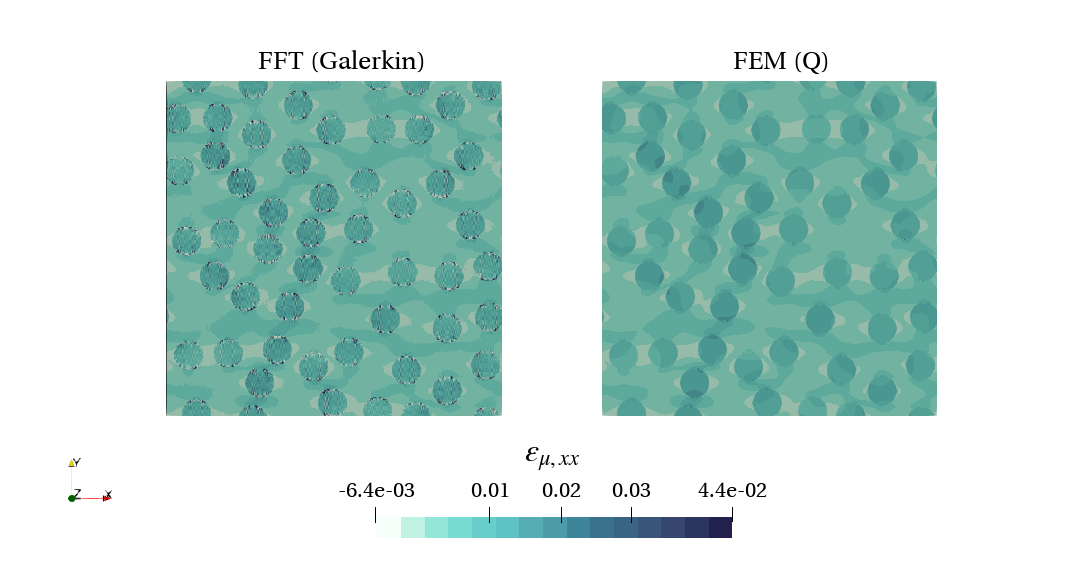
\includegraphics[width=\textwidth]{figures/linear_2D_ratio_-4_normal_strain_11}
    \caption{}
    \label{subfig:linear_2D_ratio_-4_normal_strain_11}
  \end{subfigure}
  \begin{subfigure}[b]{\textwidth}
    \centering
    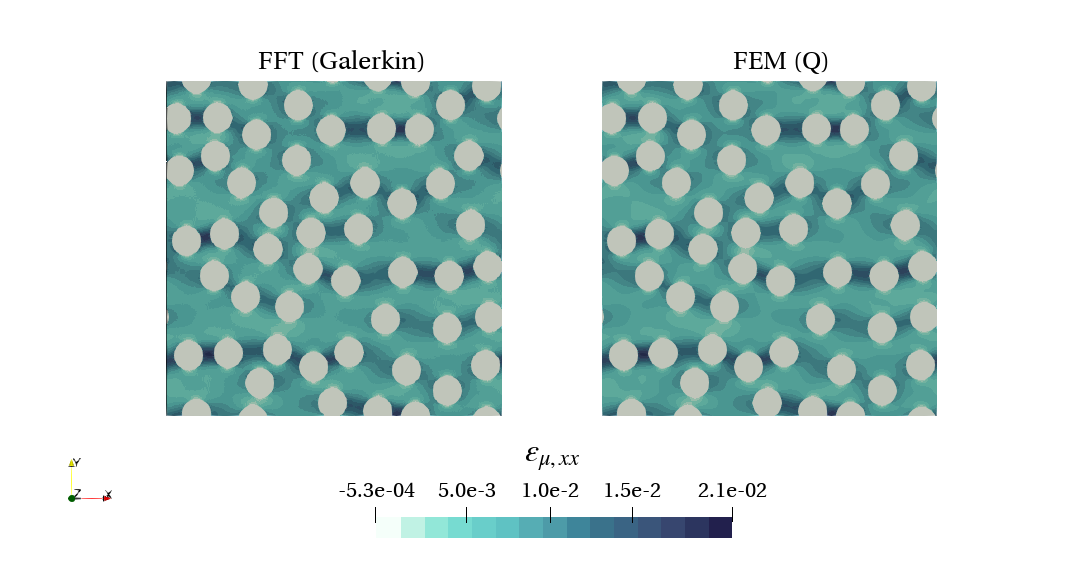
\includegraphics[width=\textwidth]{figures/linear_2D_ratio_4_normal_strain_11}
    \caption{}
    \label{subfig:linear_2D_ratio_4_normal_strain_11}
  \end{subfigure}
  \caption{Comparison between the local strain field \(\varepsilon_{\mu,xx}\) obtained using
  FFT and FEM-based homogenization approaches in the solution of the fiber-reinforced
  linear elastic composite equilibrium problem under normal strain loading conditions:
  \subref{subfig:linear_2D_ratio_-4_normal_strain_11} Stiffness ratio \(K=E_1/E_2=\num{e-4}\);
  \subref{subfig:linear_2D_ratio_4_normal_strain_11} Stiffness ratio \(K=E_1/E_2=\num{e1.5}\);
  Notation: quadratic element (Q).}
\label{fig:linear_2D_stiff_contrast_normal_strain_11}
\end{figure}

\begin{figure}[hbt]
  \centering
	\begin{subfigure}[b]{\textwidth}
    \centering
    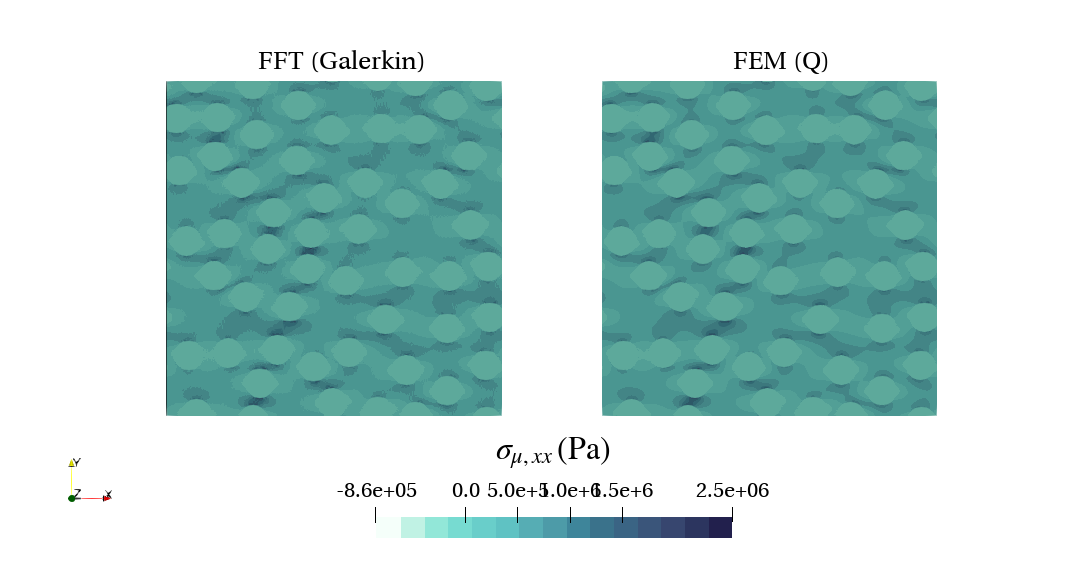
\includegraphics[width=\textwidth]{figures/linear_2D_ratio_-4_normal_stress_11}
    \caption{}
    \label{subfig:linear_2D_ratio_4_normal_stress_11}
  \end{subfigure}
  \begin{subfigure}[b]{\textwidth}
    \centering
    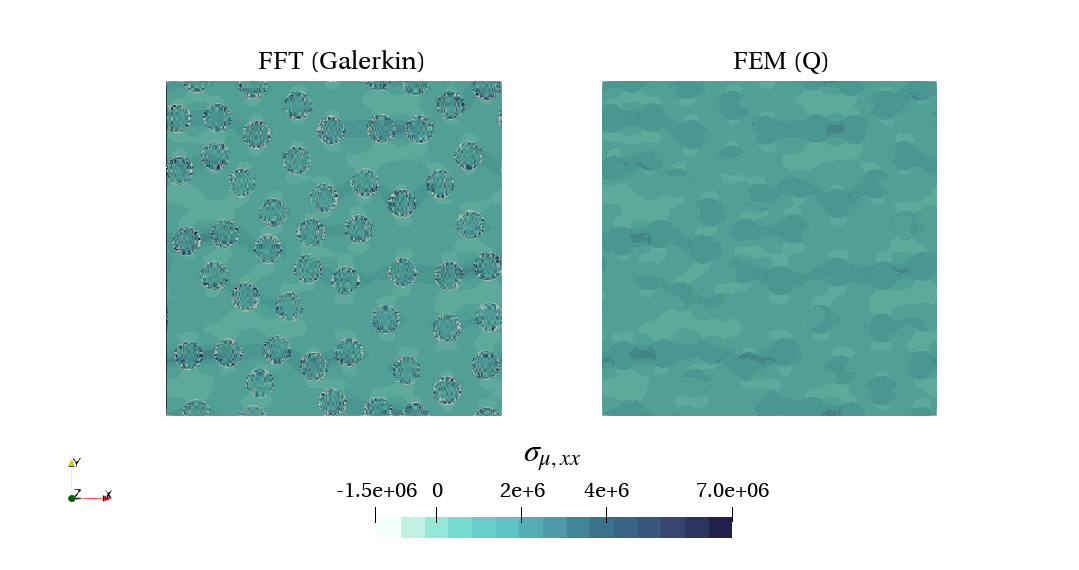
\includegraphics[width=\textwidth]{figures/linear_2D_ratio_4_normal_stress_11}
    \caption{}
    \label{subfig:linear_2D_ratio_-4_normal_stress_11}
  \end{subfigure}
  \caption{Comparison between the local stress field \(\sigma_{\mu,xx}\) obtained using
  FFT and FEM-based homogenization approaches in the solution of the fiber-reinforced
  linear elastic composite equilibrium problem under normal strain loading conditions:
  \subref{subfig:linear_2D_ratio_-4_normal_stress_11} Stiffness ratio \(K=E_1/E_2=\num{e-4}\);
  \subref{subfig:linear_2D_ratio_4_normal_stress_11} Stiffness ratio \(K=E_1/E_2=\num{e1.5}\);
  Notation: quadratic element (Q).}
\label{fig:linear_2D_stiff_contrast_normal_stress_11}
\end{figure}

\begin{figure}[hbt]
  \centering
  	\begin{subfigure}[b]{0.49\textwidth}
      \centering
      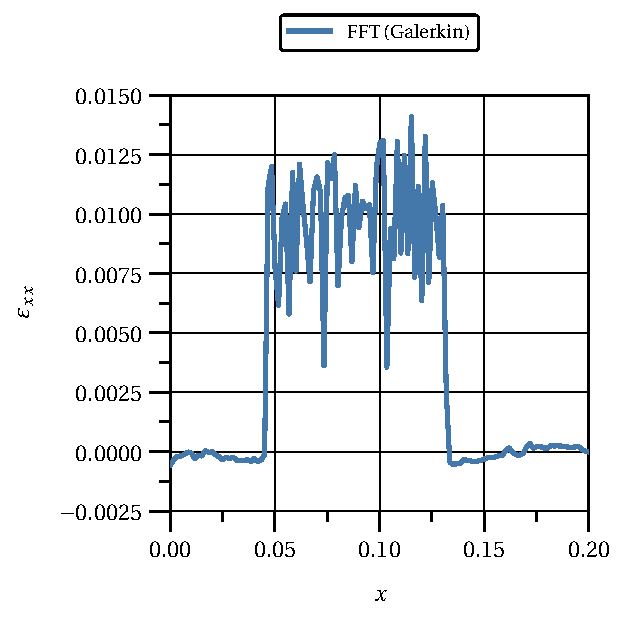
\includegraphics[width=\textwidth]{figures/linear_2D_ratio_-4_normal_strain_11_particle_1}
      \caption{}
      \label{subfig:linear_2D_ratio_-4_normal_strain_11_particle_1}
    \end{subfigure}
    \begin{subfigure}[b]{0.49\textwidth}
      \centering
      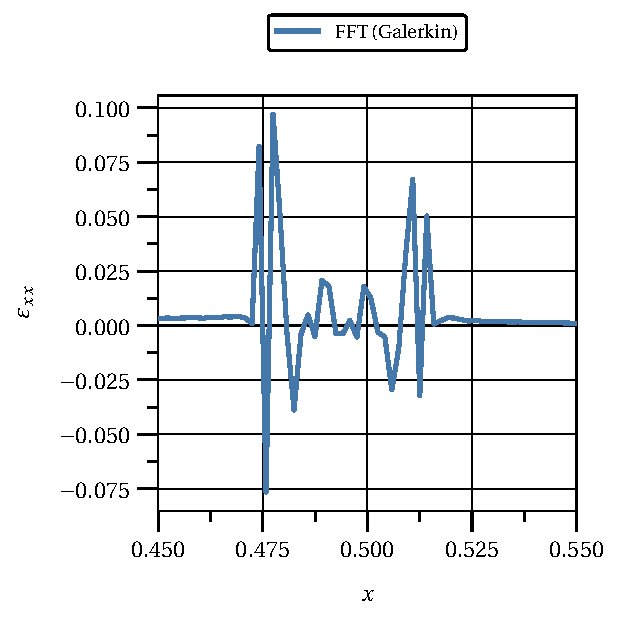
\includegraphics[width=\textwidth]{figures/linear_2D_ratio_-4_normal_strain_11_particle_2}
      \caption{}
      \label{subfig:linear_2D_ratio_-4_normal_strain_11_particle_2}
    \end{subfigure}
  \caption{Comparison between the FFT and FEM-based homogenization approaches in the solution
  of the fiber-reinforced linear elastic composite equilibrium problem under pure shear strain
  loading conditions: \subref{subfig:linear_2D_normal_stress_avg_vs_stiff_ratio} Homogenized
  stress; \subref{subfig:linear_2D_normal_stress_avg_cpu_time_vs_n_voxels} Computational time;
  Notation: linear element (L), quadratic element (Q).}
\label{fig:linear_2D_ratio_-4_normal_strain_11_particles}
\end{figure}

The numerical results of the particle-reinforced linear elastic composite equilibrium problem are shown in Figures~\ref{fig:linear_3D_normal_stiff_contrast} for the uniaxial loading case.
There is an excellent agreement between the FFT-based homogenization Galerkin scheme and the FEM-based homogenization solutions concerning the homogenized response as attested by Figure~\ref{subfig:linear_3D_normal_stress_avg_vs_stiff_ratio}.
Same cannot be said for the FFT-based homogenization Galerkin scheme as the stiffness ratio becomes more extreme.
In terms of computational performance, Figure~\ref{subfig:linear_3D_normal_stress_avg_cpu_time_vs_n_voxels} shows that the FFT-based homogenization Galerkin scheme outperforms the FEM-based homogenization with speedups from around 100 at minor stiffness contrast to around 3 at the lowest stiffness contrast, relative to the direct solver with linear finite elements.
As before, the caveat regarding the parallelization of the Python libraries still applies.
When compared with the FFT-based homogenization basic scheme, the CPU time expended differs from one to two orders of magnitude across the stiffness ranges considered, with the Galerkin scheme being slower.
It must be added that for higher stiffness ratios the WSMP-SSOR solver was not able to converge.

Concerning the local field, an excellent agreement can be observed at both high \((K=E_1/E_2=10^{1.5})\) and low \((K=E_1/E_2=\num{e-4})\) stiffness ratios in the matrix phase, as can be seen in Figures~\ref{fig:linear_3D_stiff_contrast_normal_strain_11} and \ref{fig:linear_3D_stiff_contrast_normal_stress_11}.
There is also good agreement regarding the local field in the particle phase for the strain field at the low stiffness ratio and the stress field at the high stiffness ratio.
On the other hand, the strain field at the low stiffness ratio and the strain field at the high stiffness ratio exihibt strong oscillations in the particle phase.
This mirrors the previous results concerning two dimensional microstructures.

\begin{figure}[hbt]
  \centering
  	\begin{subfigure}[b]{0.49\textwidth}
      \centering
      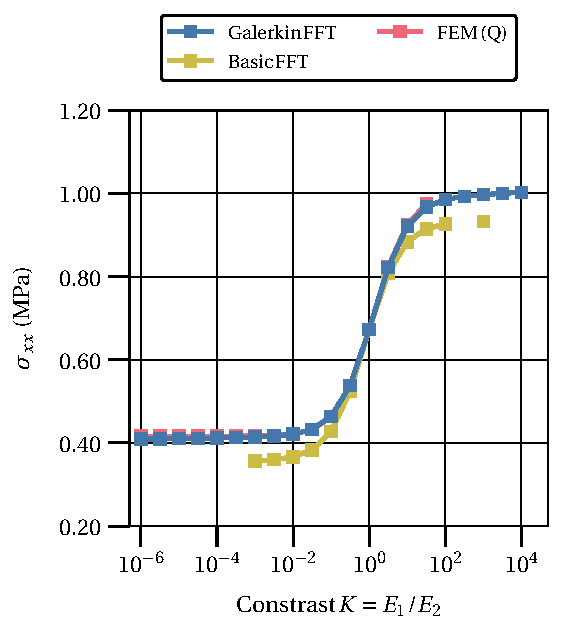
\includegraphics[width=\textwidth]{figures/linear_3D_normal_stress_avg_vs_stiff_ratio}
      \caption{}
      \label{subfig:linear_3D_normal_stress_avg_vs_stiff_ratio}
    \end{subfigure}
    \begin{subfigure}[b]{0.49\textwidth}
      \centering
      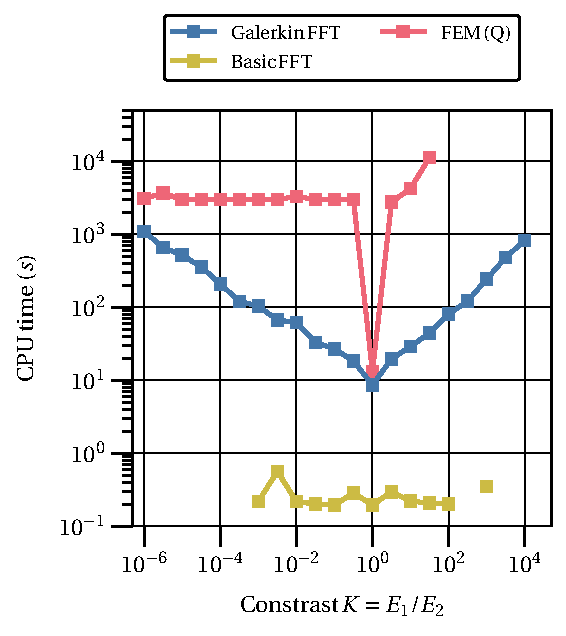
\includegraphics[width=\textwidth]{figures/linear_3D_normal_stress_avg_cpu_time_vs_n_voxels}
      \caption{}
      \label{subfig:linear_3D_normal_stress_avg_cpu_time_vs_n_voxels}
    \end{subfigure}
  \caption{Comparison between the FFT and FEM-based homogenization approaches in the solution
  of the particle-reinforced linear elastic composite equilibrium problem under normal strain
  loading conditions: \subref{subfig:linear_3D_normal_stress_avg_vs_stiff_ratio} Homogenized
  stress; \subref{subfig:linear_3D_normal_stress_avg_cpu_time_vs_n_voxels} Computational time;
  Notation: linear element (L), quadratic element (Q).}
\label{fig:linear_3D_normal_stiff_contrast}
\end{figure}

\begin{figure}[hbt]
  \centering
	\begin{subfigure}[b]{\textwidth}
    \centering
    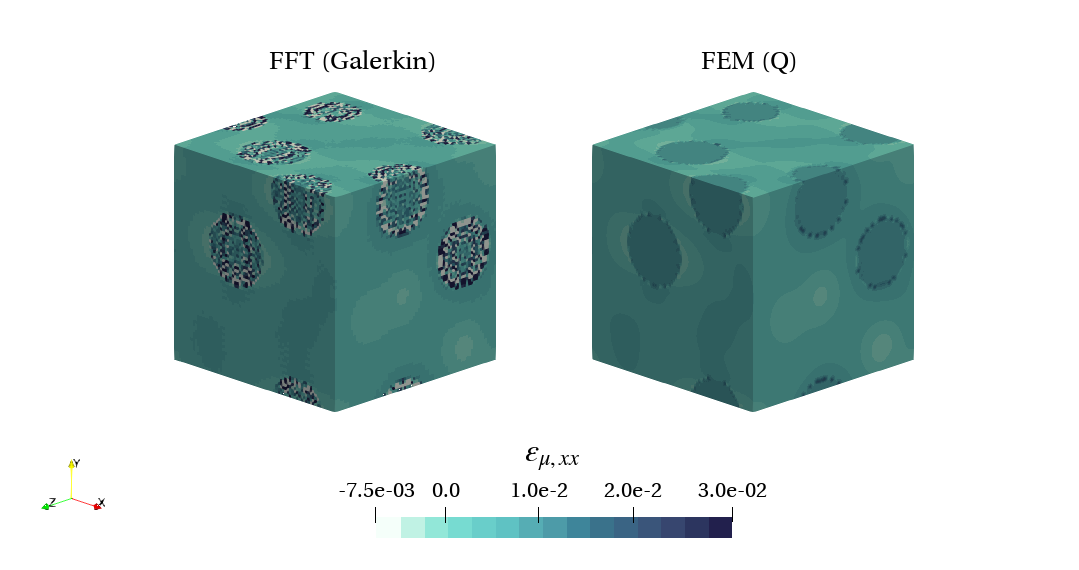
\includegraphics[width=\textwidth]{figures/linear_3D_ratio_-4_normal_strain_11}
    \caption{}
    \label{subfig:linear_3D_ratio_-4_normal_strain_11}
  \end{subfigure}
  \begin{subfigure}[b]{\textwidth}
    \centering
    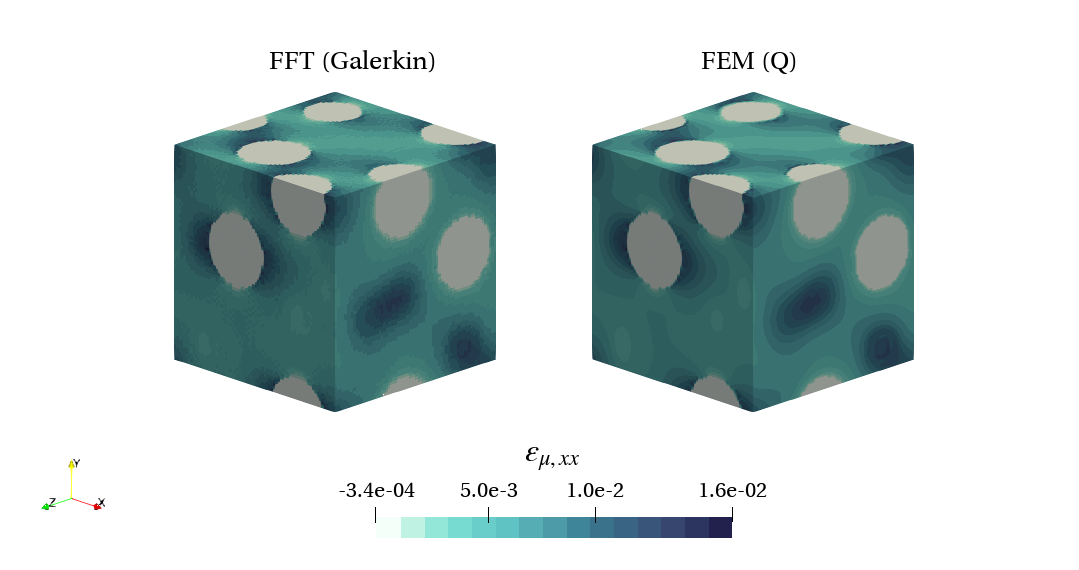
\includegraphics[width=\textwidth]{figures/linear_3D_ratio_1_5_normal_strain_11}
    \caption{}
    \label{subfig:linear_3D_ratio_1_5_normal_strain_11}
  \end{subfigure}
  \caption{Comparison between the local strain field \(\varepsilon_{\mu,xx}\) obtained using
  FFT and FEM-based homogenization approaches in the solution of the particle-reinforced
  linear elastic composite equilibrium problem under normal strain loading conditions:
  \subref{subfig:linear_3D_ratio_-4_normal_strain_11} Stiffness ratio \(K=E_1/E_2=\num{e-4}\);
  \subref{subfig:linear_3D_ratio_1_5_normal_strain_11} Stiffness ratio \(K=E_1/E_2=\num{e1.5}\);
  Notation: quadratic element (Q).}
\label{fig:linear_3D_stiff_contrast_normal_strain_11}
\end{figure}

\begin{figure}[hbt]
  \centering
	\begin{subfigure}[b]{\textwidth}
    \centering
    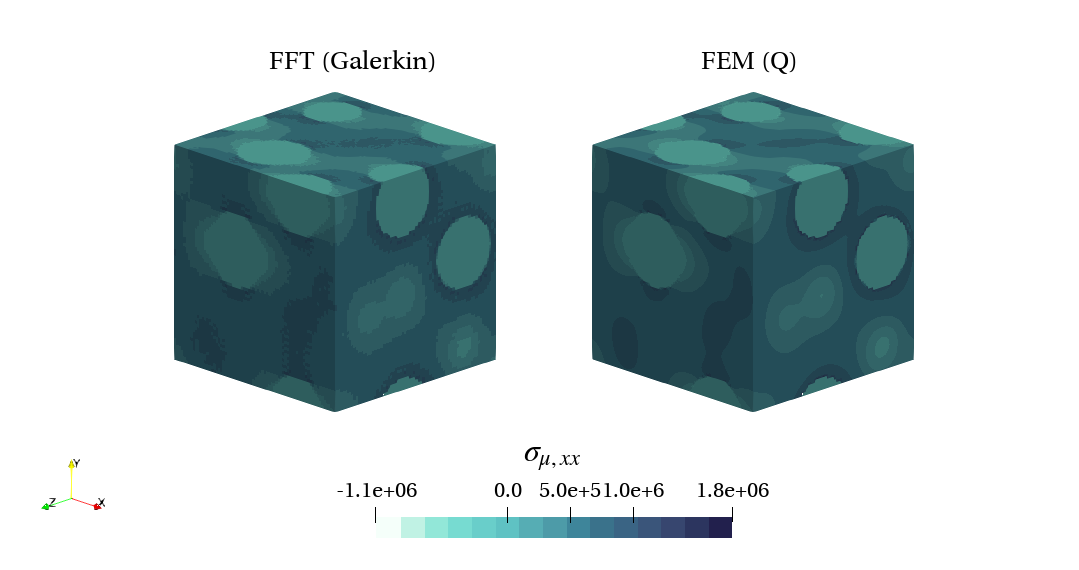
\includegraphics[width=\textwidth]{figures/linear_3D_ratio_-4_normal_stress_11}
    \caption{}
    \label{subfig:linear_3D_ratio_1_5_normal_stress_11}
  \end{subfigure}
  \begin{subfigure}[b]{\textwidth}
    \centering
    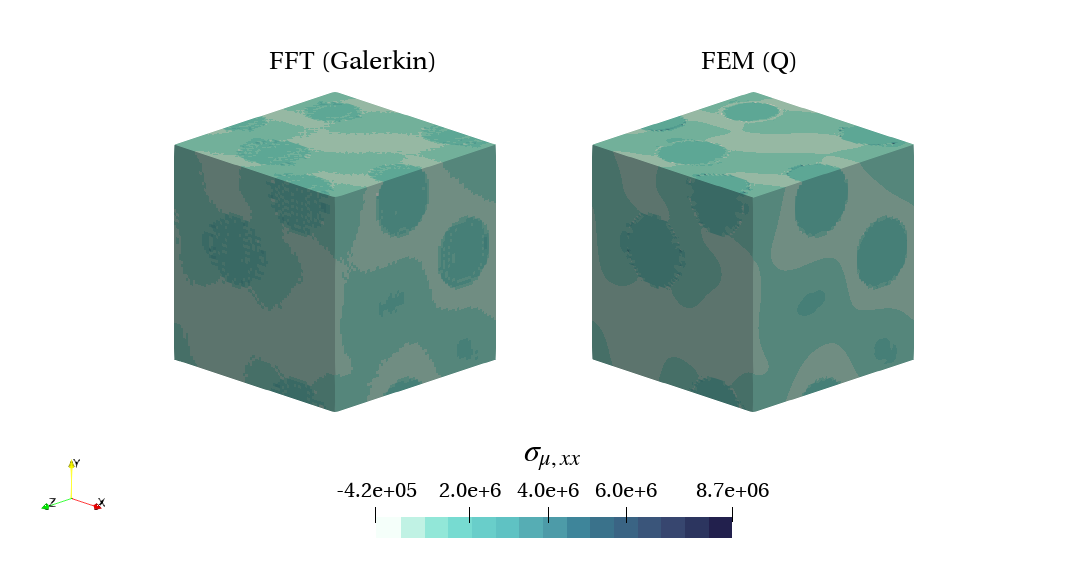
\includegraphics[width=\textwidth]{figures/linear_3D_ratio_1_5_normal_stress_11}
    \caption{}
    \label{subfig:linear_3D_ratio_-4_normal_stress_11}
  \end{subfigure}
  \caption{Comparison between the local stress field \(\sigma_{\mu,xx}\) obtained using
  FFT and FEM-based homogenization approaches in the solution of the particle-reinforced
  linear elastic composite equilibrium problem under normal strain loading conditions:
  \subref{subfig:linear_3D_ratio_-4_normal_stress_11} Stiffness ratio \(K=E_1/E_2=\num{e-4}\);
  \subref{subfig:linear_3D_ratio_1_5_normal_stress_11} Stiffness ratio \(K=E_1/E_2=\num{e1.5}\);
  Notation: quadratic element (Q).}
\label{fig:linear_3D_stiff_contrast_normal_stress_11}
\end{figure}


\FloatBarrier

\subsection{Large strain}

\paragraph{Accuracy validation}

\subparagraph{Hencky}

\begin{figure}[hbt]
  \centering
	\begin{subfigure}[b]{0.49\textwidth}
    \centering
    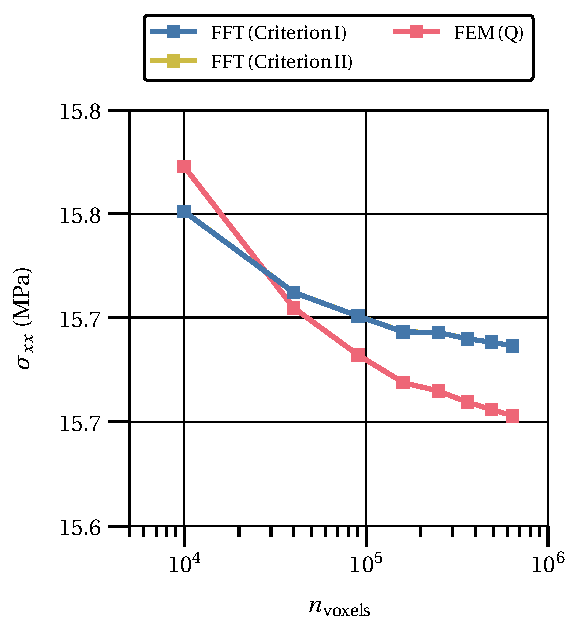
\includegraphics[width=\textwidth]{figures/hencky_2D_normal_homo_stress_11_vs_n_voxels}
    \caption{}
    \label{subfig:hencky_2D_normal_homo_stress_11_vs_n_voxels}
  \end{subfigure}
  \begin{subfigure}[b]{0.49\textwidth}
    \centering
    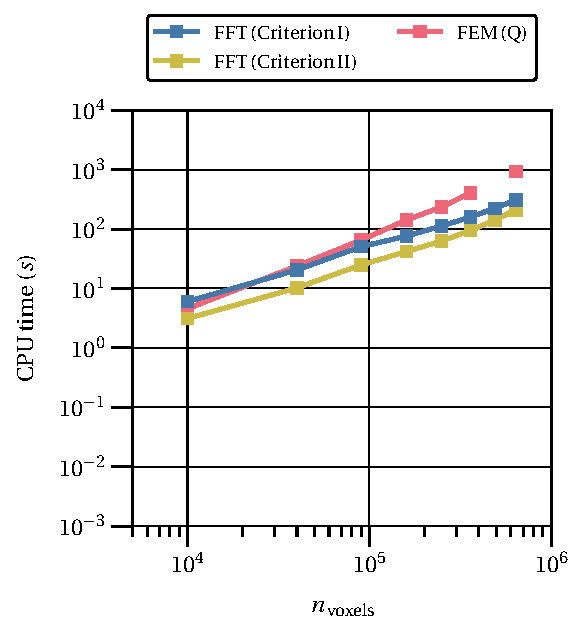
\includegraphics[width=\textwidth]{figures/hencky_2D_normal_cpu_time_vs_n_voxels}
    \caption{}
    \label{subfig:hencky_2D_normal_cpu_time_vs_n_voxels}
  \end{subfigure}
  \begin{subfigure}[b]{\textwidth}
    \centering
    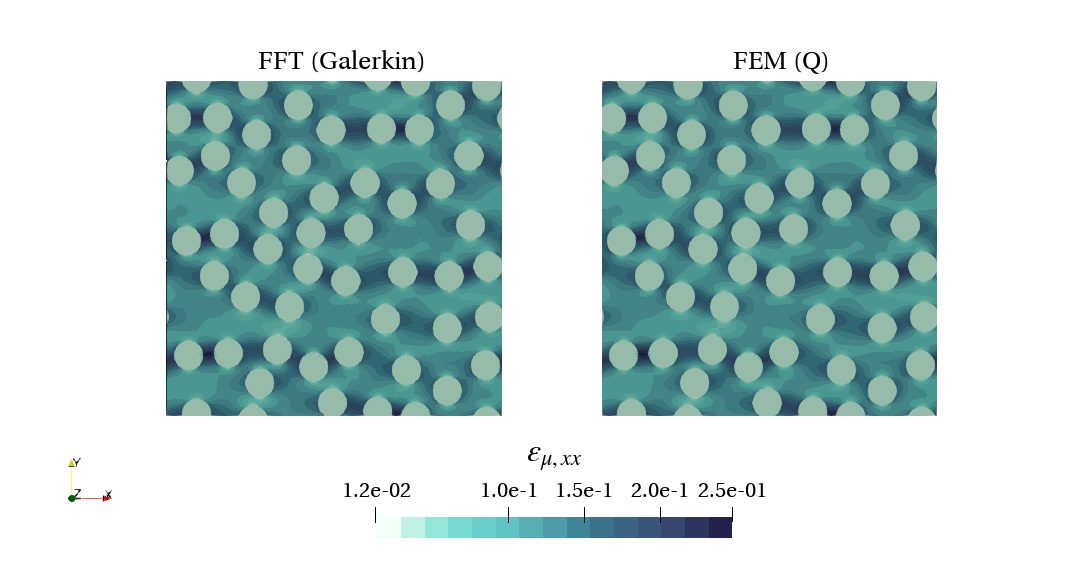
\includegraphics[width=\textwidth]{figures/hencky_2D_normal_strain_11}
    \caption{}
    \label{subfig:hencky_2D_normal_strain_11}
  \end{subfigure}
  \caption{Comparison between the Criterion I and II for FFT-based homogenization approaches, Galerkin and Basic, in the
  solution of the particle-reinforced hencky elastic composite equilibrium problem under uniaxial
  strain loading conditions: \subref{subfig:hencky_2D_shear_comparison_crit_homo_stress_12_vs_n_voxels} Homogenized stress; \subref{subfig:hencky_2D_shear_comparison_crit_cpu_time_vs_n_voxels} Computational time.}
\label{fig:hencky_2D_normal}
\end{figure}

\begin{figure}[hbt]
  \centering
	\begin{subfigure}[b]{0.49\textwidth}
    \centering
    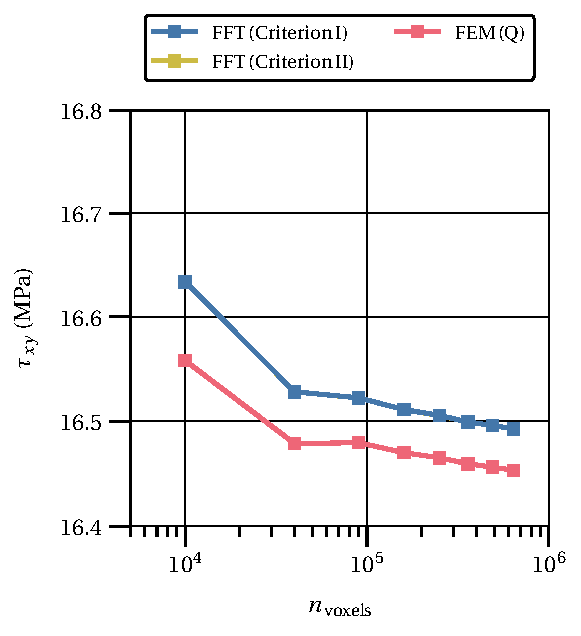
\includegraphics[width=\textwidth]{figures/hencky_2D_shear_homo_stress_12_vs_n_voxels}
    \caption{}
    \label{subfig:hencky_2D_shear_homo_stress_12_vs_n_voxels}
  \end{subfigure}
  \begin{subfigure}[b]{0.49\textwidth}
    \centering
    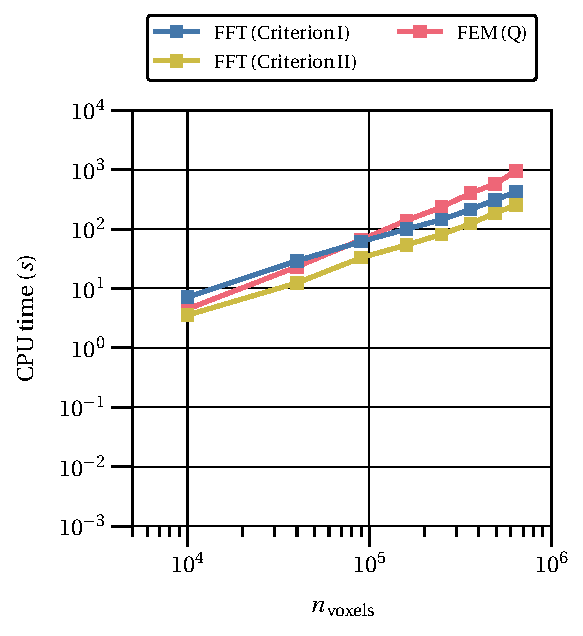
\includegraphics[width=\textwidth]{figures/hencky_2D_shear_cpu_time_vs_n_voxels}
    \caption{}
    \label{subfig:hencky_2D_shear_cpu_time_vs_n_voxels}
  \end{subfigure}
  \begin{subfigure}[b]{\textwidth}
    \centering
    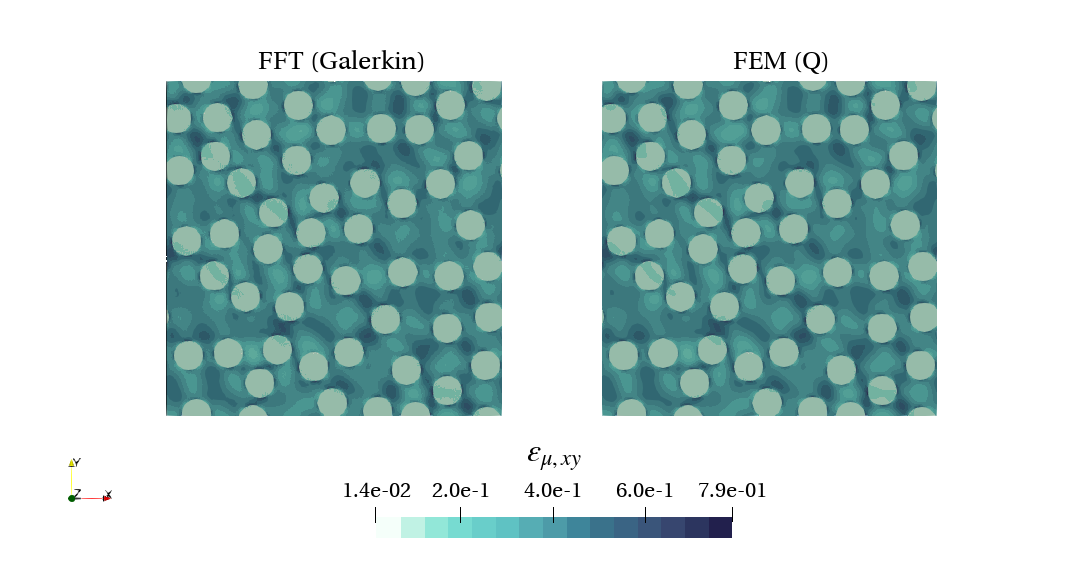
\includegraphics[width=\textwidth]{figures/hencky_2D_shear_strain_12}
    \caption{}
    \label{subfig:hencky_2D_shear_strain_12}
  \end{subfigure}
  \caption{f}
\label{fig:hencky_2D_shear}
\end{figure}

\begin{figure}[hbt] % incomplete
\label{fig:hencky_mat_res_2D_normal}
\end{figure}

\begin{figure}[hbt] % incomplete
\label{fig:hencky_mat_res_2D_shear}
\end{figure}

% No convergence study is done due time, memory constrainst so 70x70x70

\begin{figure}[hbt] % incomplete
\label{fig:hencky_mat_res_3D_normal}
\end{figure}

\begin{figure}[hbt] % incomplete
\label{fig:hencky_mat_res_3D_shear}
\end{figure}

\FloatBarrier

\subparagraph{Saint Venant-Kirchhoff model}

\begin{figure}[hbt]
  \centering
	\begin{subfigure}[b]{0.49\textwidth}
    \centering
    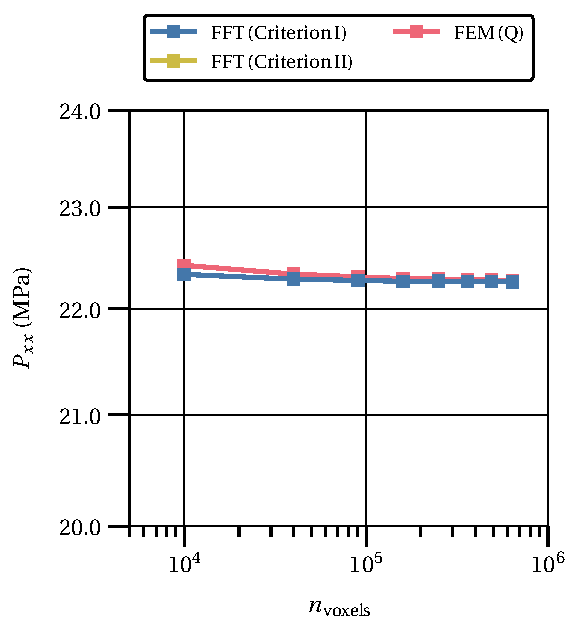
\includegraphics[width=\textwidth]{figures/svk_2D_normal_homo_stress_11_vs_n_voxels}
    \caption{}
    \label{subfig:svk_2D_normal_homo_stress_11_vs_n_voxels}
  \end{subfigure}
  \begin{subfigure}[b]{0.49\textwidth}
    \centering
    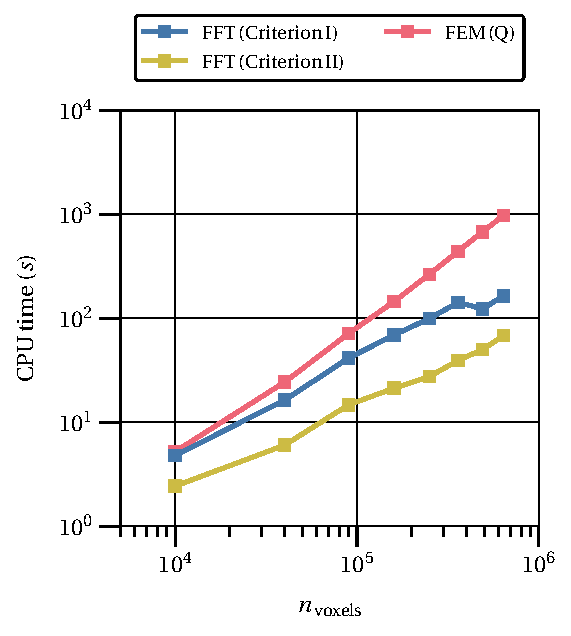
\includegraphics[width=\textwidth]{figures/svk_2D_normal_cpu_time_vs_n_voxels}
    \caption{}
    \label{subfig:svk_2D_normal_cpu_time_vs_n_voxels}
  \end{subfigure}
  \begin{subfigure}[b]{\textwidth}
    \centering
    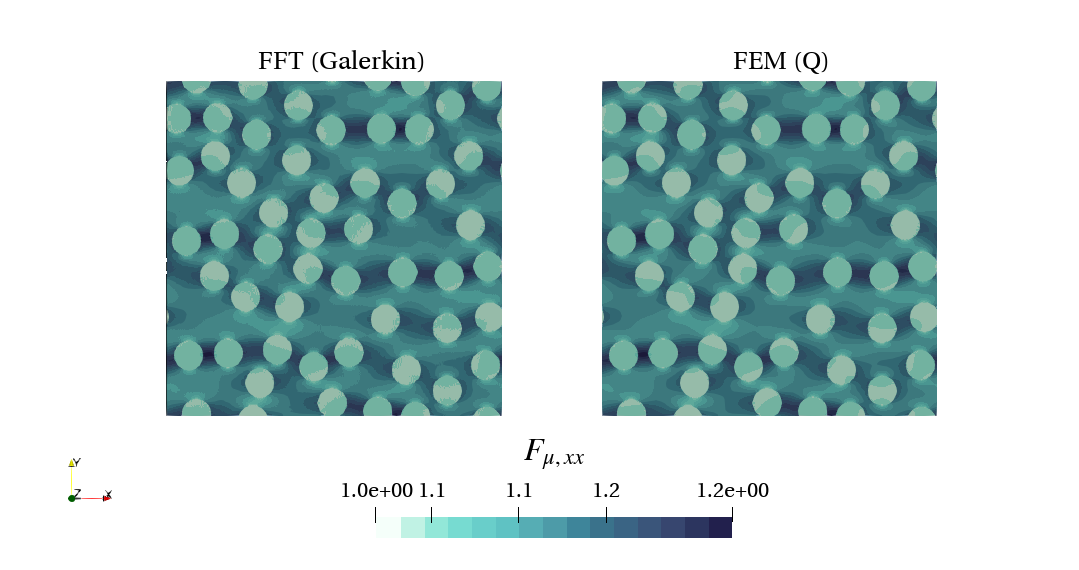
\includegraphics[width=\textwidth]{figures/svk_2D_normal_strain_11}
    \caption{}
    \label{subfig:svk_2D_normal_strain_11}
  \end{subfigure}
  \caption{Comparison between the Criterion I and II for FFT-based homogenization
  approaches, Galerkin and Basic, in the solution of the particle-reinforced svk elastic
  composite equilibrium problem under uniaxial strain loading conditions:
  \subref{subfig:svk_2D_normal_comparison_crit_homo_stress_11_vs_n_voxels} Homogenized
  stress; \subref{subfig:svk_2D_normal_comparison_crit_cpu_time_vs_n_voxels} Computational
  time.}
\label{fig:svk_2D_normal}
\end{figure}

\FloatBarrier

\paragraph{Extreme stiffness ratios between phases}

\subparagraph{Hencky}

\subparagraph{Saint Venant-Kirchhoff model}

\begin{figure}[hbt]
  \centering
	\begin{subfigure}[b]{0.49\textwidth}
    \centering
    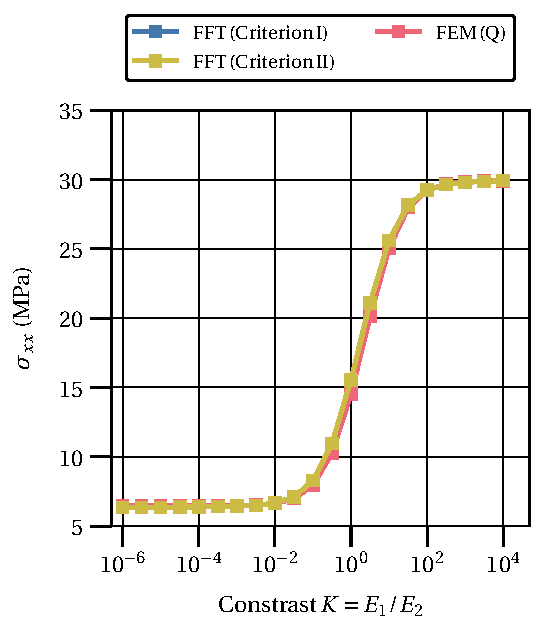
\includegraphics[width=\textwidth]{figures/svk_2D_normal_stress_avg_vs_stiff_ratio}
    \caption{}
    \label{subfig:svk_2D_normal_stress_avg_vs_stiff_ratio}
  \end{subfigure}
  \begin{subfigure}[b]{0.49\textwidth}
    \centering
    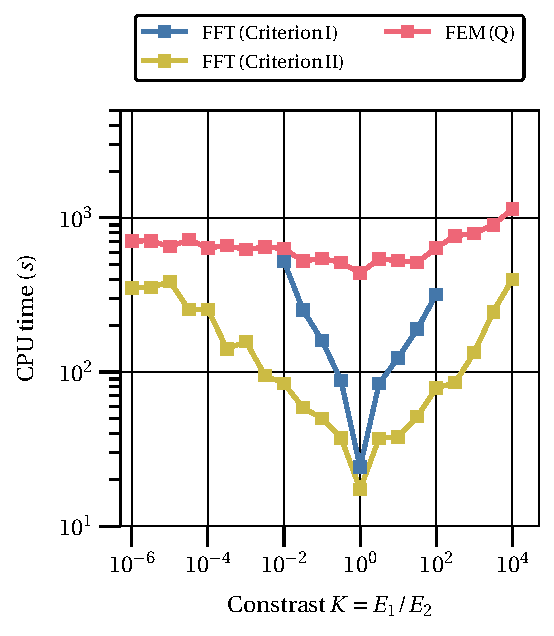
\includegraphics[width=\textwidth]{figures/svk_2D_normal_stress_avg_cpu_time_vs_n_voxels}
    \caption{}
    \label{subfig:svk_2D_normal_stress_avg_cpu_time_vs_n_voxels}
  \end{subfigure}
  \caption{Comparison between the Criterion I and II for FFT-based homogenization approaches, Galerkin and Basic, in the
  solution of the particle-reinforced svk elastic composite equilibrium problem under uniaxial
  strain loading conditions: \subref{subfig:svk_3D_normal_comparison_crit_homo_stress_11_vs_n_voxels} Homogenized stress; \subref{subfig:svk_3D_normal_comparison_crit_cpu_time_vs_n_voxels} Computational time.}
\label{fig:svk_2D_normal_stiff_contrast}
\end{figure}

\begin{figure}[hbt]
  \centering
	\begin{subfigure}[b]{\textwidth}
    \centering
    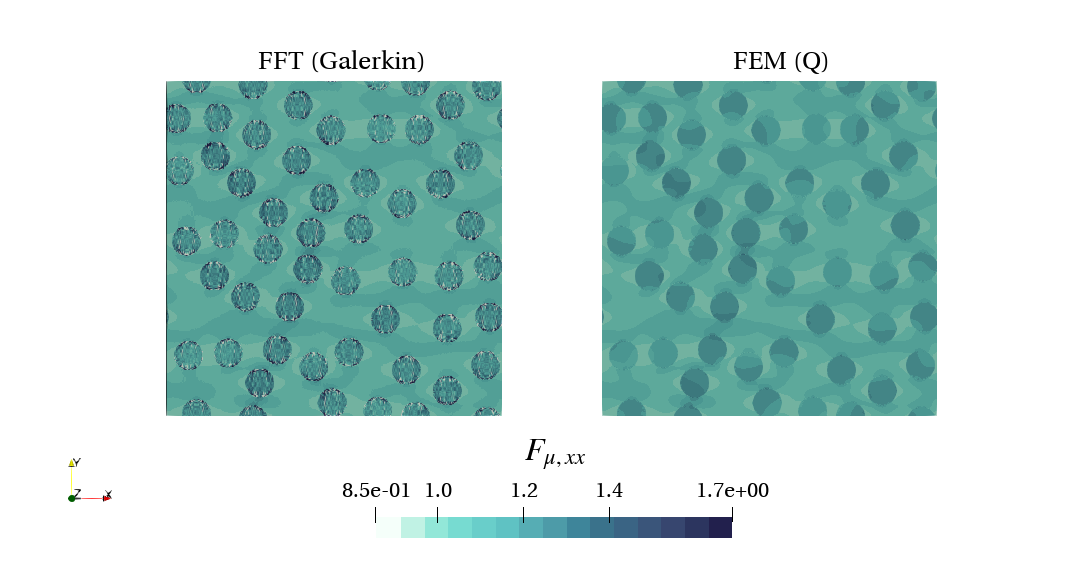
\includegraphics[width=\textwidth]{figures/svk_2D_ratio_-4_normal_strain_11}
    \caption{}
    \label{subfig:svk_2D_ratio_4_normal_strain_11}
  \end{subfigure}
  \begin{subfigure}[b]{\textwidth}
    \centering
    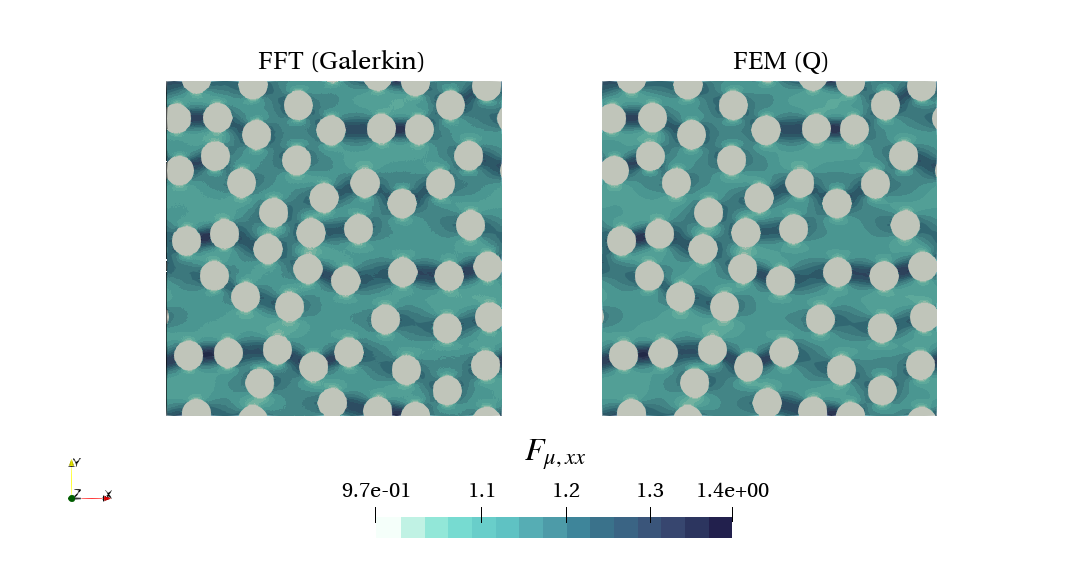
\includegraphics[width=\textwidth]{figures/svk_2D_ratio_4_normal_strain_11}
    \caption{}
    \label{subfig:svk_2D_ratio_-4_normal_strain_11}
  \end{subfigure}
  \caption{Comparison between the Criterion I and II for FFT-based homogenization approaches, Galerkin and Basic, in the
  solution of the particle-reinforced svk elastic composite equilibrium problem under uniaxial
  strain loading conditions: \subref{subfig:svk_3D_normal_comparison_crit_homo_stress_11_vs_n_voxels} Homogenized stress; \subref{subfig:svk_3D_normal_comparison_crit_cpu_time_vs_n_voxels} Computational time.}
\label{fig:svk_2D_stiff_contrast_normal_strain_11}
\end{figure}

\FloatBarrier
